\documentclass[a4paper]{article}
\usepackage{graphicx}
\usepackage{amsmath, amsfonts, geometry, float, listings, enumerate, multicol}
\usepackage{multicol, float, colortbl}
\usepackage{lipsum}
\usepackage{tikz, titlesec, parskip}
\usepackage{tikz,pgfplots, circuitikz}
\usepackage{epsfig,graphicx,amsthm,amsmath}
\usepackage{wrapfig}
\usepackage{subfigure}
\usepackage{caption}
\usepackage{subfigure}
\usepackage{graphicx}
\usepackage{pythontex} 
\usepackage{matlab-prettifier}
\usepackage{tabularx}
\usepackage{media9}
\usepackage[utf8]{inputenc}
\usepackage{color}
\usepackage[symbol]{footmisc}
\usepackage{lipsum}\usepackage{parskip}\usepackage{booktabs}
\usepackage{soul}

\usepackage{caption, enumitem}
\definecolor{forest}{RGB}{34,139,34}
\definecolor{c1}{RGB}{0,128,255}
\definecolor{c2}{RGB}{0,204,102}
\definecolor{c3}{RGB}{0,128,128}
\definecolor{c4}{RGB}{255,102,102}
\definecolor{c5}{RGB}{130,50,220}
\definecolor{c6}{RGB}{0,204,102}
\definecolor{c7}{RGB}{255,153,51}
\definecolor{c8}{RGB}{153,153,255}
\definecolor{c9}{RGB}{160,160,160}
\definecolor{c0}{RGB}{240,200,0}
\usetikzlibrary{arrows,calc,positioning}
\tikzset{
	block/.style = {draw, rectangle,
		minimum height=1cm,
		minimum width=2cm},
	input/.style = {coordinate,node distance=1cm},
	output/.style = {coordinate,node distance=4cm},
	arrow/.style={draw, -latex,node distance=2cm},
	pinstyle/.style = {pin edge={latex-, black,node distance=2cm}},
	sum/.style = {draw, circle, node distance=1cm},
}

\usepackage{relsize}
\usepackage[pagebackref=false,colorlinks,linkcolor=forest,urlcolor= blue,citecolor=blue]{hyperref}

\titlespacing{\section}{0pt}{10pt}{0pt}
\titlespacing{\subsection}{0pt}{10pt}{0pt}
\titlespacing{\subsubsection}{0pt}{10pt}{0pt}

\usetikzlibrary{calc,patterns,through}
\newcommand{\arcangle}{%
	\mathord{<\mspace{-9mu}\mathrel{)}\mspace{2mu}}%
}

\newcommand{\Cross}{$\mathbin{\tikz [x=1.4ex,y=1.4ex,line width=.2ex] \draw (0,0) -- (1,1) (0,1) -- (1,0);}$}%


\renewcommand{\baselinestretch}{1.2}
\geometry{
	a4paper,
	total={170mm,257mm},
	left=20mm,
	top=20mm,
}

\usepackage{hyperref}
\hypersetup{
	colorlinks=true,
	linkcolor=forest,
	filecolor=magenta,      
	urlcolor=cyan,
	pdftitle={Overleaf Example},
	pdfpagemode=FullScreen,
}

\usepackage{fancyhdr}
\pagestyle{fancy}
\fancyhf{}
\rhead{\textbf{ Farzan Aghaei }}
\lhead{\textbf{ Assignment 4 }}
\lfoot{(\space\textbf{\thepage}\space)}
\rfoot{\textbf{Data Networks }}
\renewcommand{\headrulewidth}{1pt}
\renewcommand{\footrulewidth}{1pt}

%\renewcommand{\thefootnote}{{footnote}}


\begin{document}
	\begin{minipage}{0.65\textwidth}
		\begin{center}
			\normalsize
			‫		In the name of Allah\\
			\vspace{0.5cm}
			\huge
			\textbf{Data Networks} \\
			\vspace{0.2cm}
			\LARGE
			Prof. Mohammad Reza Pakravan \\
			\vspace{0.5cm}
			\Large
			Assignment 4\\
			\vspace{0.6cm}
			Farzan Aghaei 401101202
			\vspace{0.2cm}
		\end{center}
		\normalsize
	\end{minipage}
	\begin{minipage}{0.35\textwidth}
		\begin{flushleft}
			\centering
			
\includegraphics[width=0.7\textwidth]{Shariflogo.jpg}\\ \large
			
			\vspace{0.4cm}
			Sharif University of Technology\\
			\vspace{0.2cm}
			Electrical Engineering Department\\
			\vspace{0.2cm}
		\end{flushleft}
	\end{minipage}
	
	\rule[0.1\baselineskip]{\textwidth}{1pt}
	
	\section{Analyzing Protocols Using Wireshark}
	
	\subsection{Analyze IP Protocol}
	
	\subsubsection{Simulation Scenario: Ping Your Gateway and Analyze IP Packets}
	
	I first started capturing traffic on WiFi interface. After that I opened the command prompt and then used the \textit{ipconfig} command to find out that my default gateway IP's address is \colorbox{lime}{192.168.100.1}. Then using \textit{ping 192.168.100.1} I ran a ping command in that gateway and after it completed I stopped the capture.
	
	The results of the process above are shown in the following figure.
	
	\begin{figure}[!h]
		\centering
		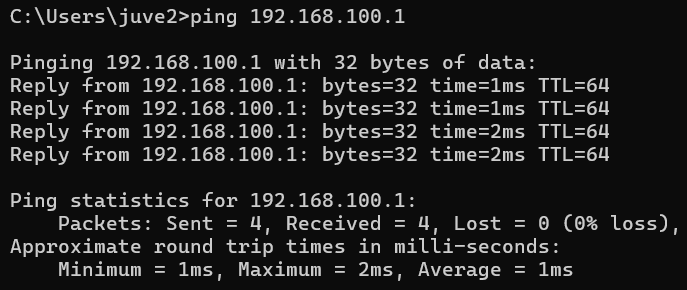
\includegraphics[width=0.7\linewidth]{screenshot001}
		\caption{default gateway ping process result}
		\label{fig:screenshot001}
	\end{figure}
	
	Next I filtered the ICMP packets, chose the first Echo Request one and then expanded its IP section which can be observed below.
	
	\begin{figure}[!h]
		\centering
		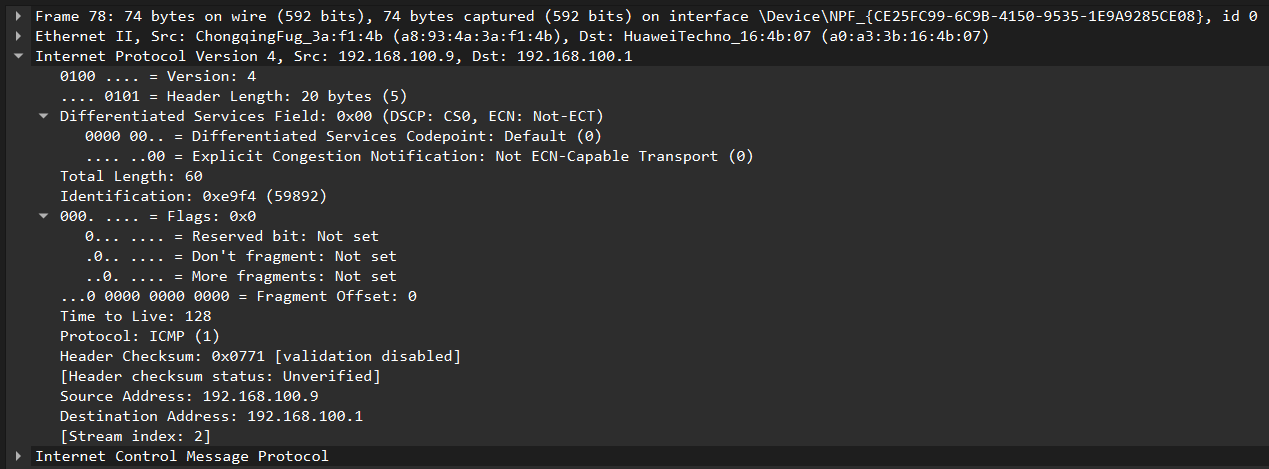
\includegraphics[width=0.7\linewidth]{screenshot002}
		\caption{The IP section of the first captured ICMP packet}
		\label{fig:screenshot002}
	\end{figure}
	
	\pagebreak
	
	\subsubsection{Questions: IP Header Field Analysis}
	
	\begin{enumerate}
		\item \textbf{Header Length:} What is the header length in bytes?
		
		As it can be seen in \ref{fig:screenshot002}, the header length is 5 bytes.
		
		\item \textbf{Type of Service (DSCP/ECN):} What value is set? What is the purpose of this field?
		
		The value set to this field is 0x00. This field is used for Quality of Service. DSCP specifies packet priority, and ECN is used for congestion notification in networks.
		
		\item \textbf{Total Length:} What is the size of the entire IP packet?
		
		The total length is 60 bytes.
		
		\item \textbf{Identification:} What is the purpose of this field?
		
		This filed is set to 0xe9f4 (59892) .This field is used to uniquely identify fragments of an original IP datagram. It helps the receiving system reassemble packets that have been fragmented during transmission.
		
		\item \textbf{Flags and Fragment Offset:} Are any flags set? What do they mean?
		
		The flags field is set to 0x0 which tells us that there are no flags set. This means that no fragmentation is occurring, this packet is not fragmented and there are no restrictions on fragmentation.
		
		\item \textbf{Time to Live (TTL):} What is the TTL value? Why is this important?
		
		The TTL value is 128. TTL limits the lifetime of a packet to prevent it from circulating indefinitely in case of routing loops. Each router that forwards the packet decreases the TTL by 1; when it reaches 0, the packet is discarded.
		 
		\item \textbf{Protocol:} Which Layer 4 protocol is encapsulated in this IP packet?
		
		The protocol is ICMP (1). It is commonly used for diagnostics (e.g., ping).
		
		\item \textbf{Source and Destination IPs:} Do these match your IP and gateway?
		
		The source address is \colorbox{lime}{192.168.100.9} and the destination address is \colorbox{lime}{192.168.100.1} and they match my computer's IP and gateway. 
		 
	\end{enumerate}
	
	\subsection{Analyze DHCP Protocol}
	
	\subsubsection{Simulation Scenario}
	
	Again in this part I started capturing packets on my WiFi interface. Then I released and renewed my IP address to initiate DHCP exchange using the commands \textit{ipconfig /release} and \textit{ipconfig /renew}.
	
	\begin{figure}[!h]
		\centering
		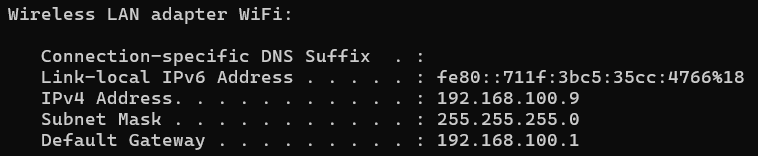
\includegraphics[width=0.7\linewidth]{screenshot004}
		\caption{The Wireless LAN adapter WiFi after release and renew}
		\label{fig:screenshot004}
	\end{figure}
	
	After a few seconds I stopped the packet capturing process and applied the dhcp display filter on the captured packets.
	
	\begin{figure}[!h]
		\centering
		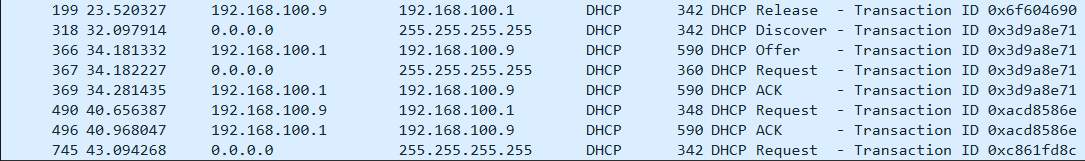
\includegraphics[width=0.7\linewidth]{screenshot003}
		\caption{The filtered DHCP packets}
		\label{fig:screenshot003}
	\end{figure}
	
	We can see the packet sequence Discover, Offer, Request, Acknowledgment.
	
	\subsubsection{Questions}
	
	\begin{figure}[!htb]
		\begin{minipage}{0.49\textwidth}
			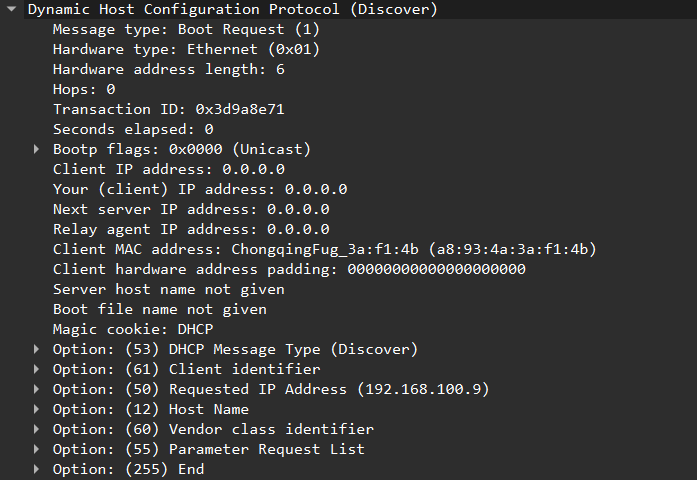
\includegraphics[width=\linewidth]{screenshot006}
		\end{minipage}\hfill
		\begin{minipage}{0.49\textwidth}
			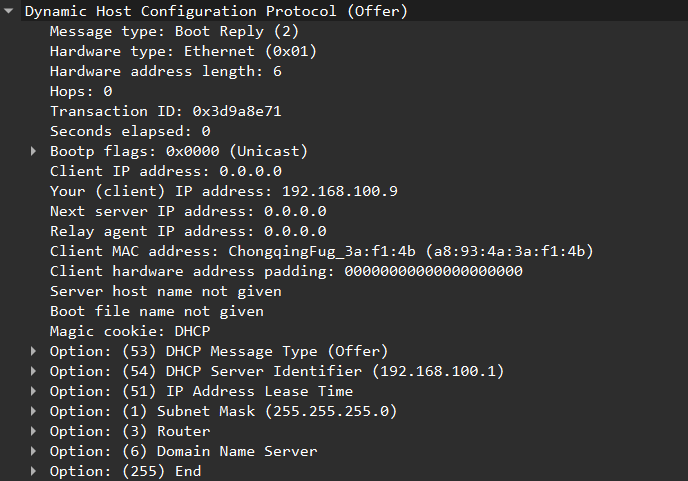
\includegraphics[width=\linewidth]{screenshot005}
		\end{minipage}\hfill
		\caption{DHCP Discover and Offer packet details}
		\label{1}
	\end{figure}
	\begin{figure}[!htb]
		\begin{minipage}{0.49\textwidth}
			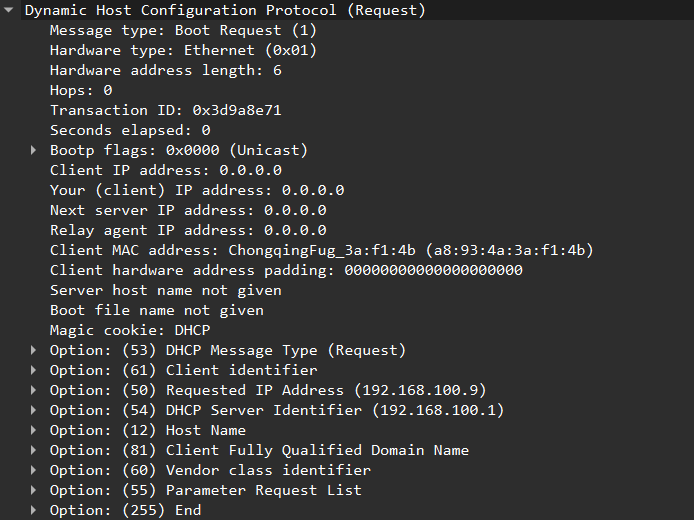
\includegraphics[width=\linewidth, height=0.69\textwidth]{screenshot007}
		\end{minipage}\hfill
		\begin{minipage}{0.49\textwidth}
			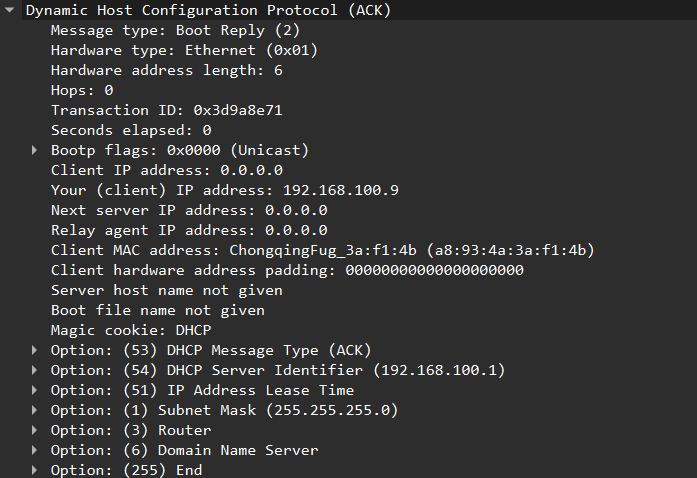
\includegraphics[width=\linewidth]{screenshot008}
		\end{minipage}\hfill
		\caption{DHCP Request and Acknowledgment packet details}
		\label{2}
	\end{figure}
	
	\begin{enumerate}
		\item What is the MAC address and IP address of your machine as shown in the DHCP packets?
		
		\begin{itemize}
			\item Discover:
				
				MAC address: \colorbox{lime}{a8:93:4a:3a:f1:4b} \qquad\qquad my (client) IP address: \colorbox{lime}{0.0.0.0}
				
			\item Offer:
			
				MAC address: \colorbox{lime}{a8:93:4a:3a:f1:4b} \qquad\qquad my (client) IP address: \colorbox{lime}{192.168.100.9}
				
			\item Request:
			
				MAC address: \colorbox{lime}{a8:93:4a:3a:f1:4b} \qquad\qquad my (client) IP address: \colorbox{lime}{0.0.0.0}
			
			\item ACK:
			
				MAC address: \colorbox{lime}{a8:93:4a:3a:f1:4b} \qquad\qquad my (client) IP address: \colorbox{lime}{192.168.100.9}
		\end{itemize}
		
		\item Explain the purpose of the packet (e.g., DHCP Discover, Offer, Request, or Acknowledgment).
		
		The client sends a DHCP Discover packet to find available DHCP servers on the network. It’s a broadcast packet \colorbox{lime}{255.255.255.255} since the client doesn’t have an IP address yet. Then the DHCP servers that receive the Discover respond with a DHCP Offer packet. This packet includes an available IP address, subnet mask, gateway, lease time, and possibly other info. The client responds to the offer by sending a DHCP Request packet, telling the chosen DHCP server that it wants to use the offered IP address. This is also broadcast, so all DHCP servers see it. The chosen DHCP server finalizes the process by sending a DHCP ACK packet to the client. This confirms the IP address assignment and provides configuration details.
		
	\end{enumerate}
	
	\subsubsection{Simulation Scenario: DHCP Server on Laptop via Mobile Hotspot}
	
	In this experiment I enabled the mobile hotspot of my laptop after beginning to capture packet on the interface "Local Area Connection* 2". Then I connected my phone to the hotspot and after a few seconds stopped capturing. The filtered DHCP packets are shown in the figure below.
	
	\begin{figure}[h!]
		\centering
		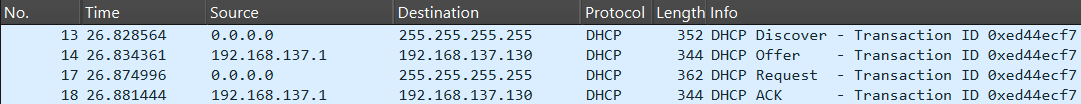
\includegraphics[width=0.7\linewidth]{screenshot013}
		\caption{}
		\label{fig:screenshot013}
	\end{figure}
	
	\subsubsection{Questions}
	
	\begin{figure}[!htb]
		\begin{minipage}{0.49\textwidth}
			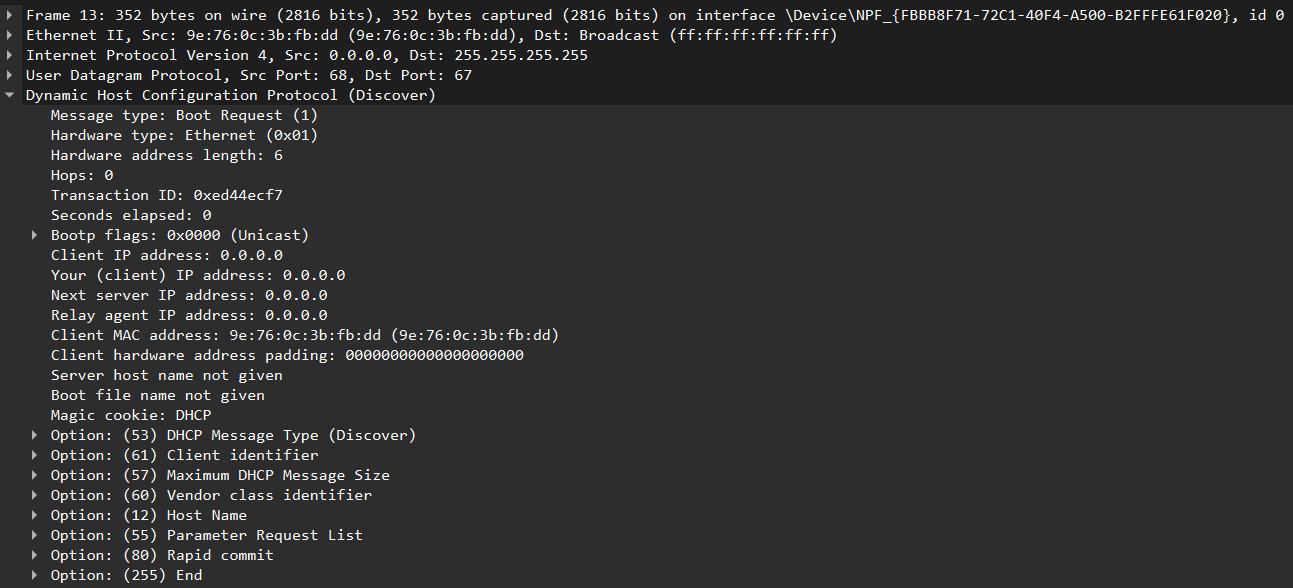
\includegraphics[width=\linewidth, height=0.5\textwidth]{screenshot009}
		\end{minipage}\hfill
		\begin{minipage}{0.49\textwidth}
			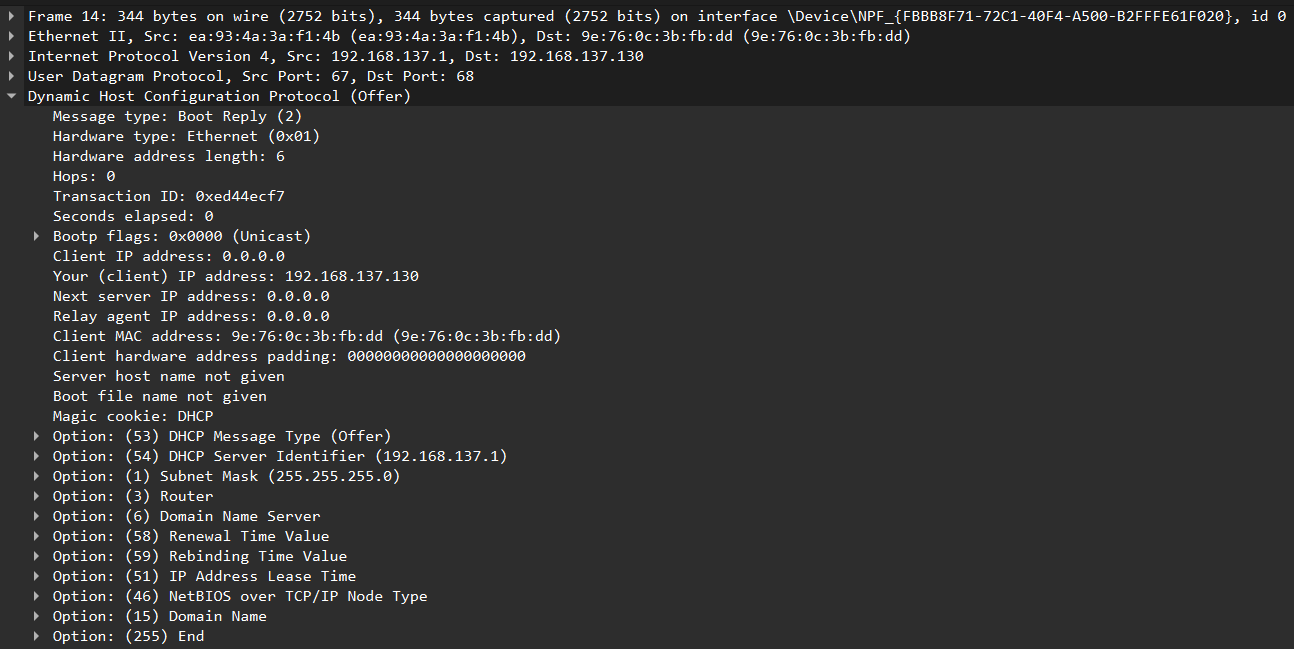
\includegraphics[width=\linewidth]{screenshot010}
		\end{minipage}\hfill
		\caption{DHCP Discover and Offer packet details}
		\label{1}
	\end{figure}
	\begin{figure}[!htb]
		\begin{minipage}{0.49\textwidth}
			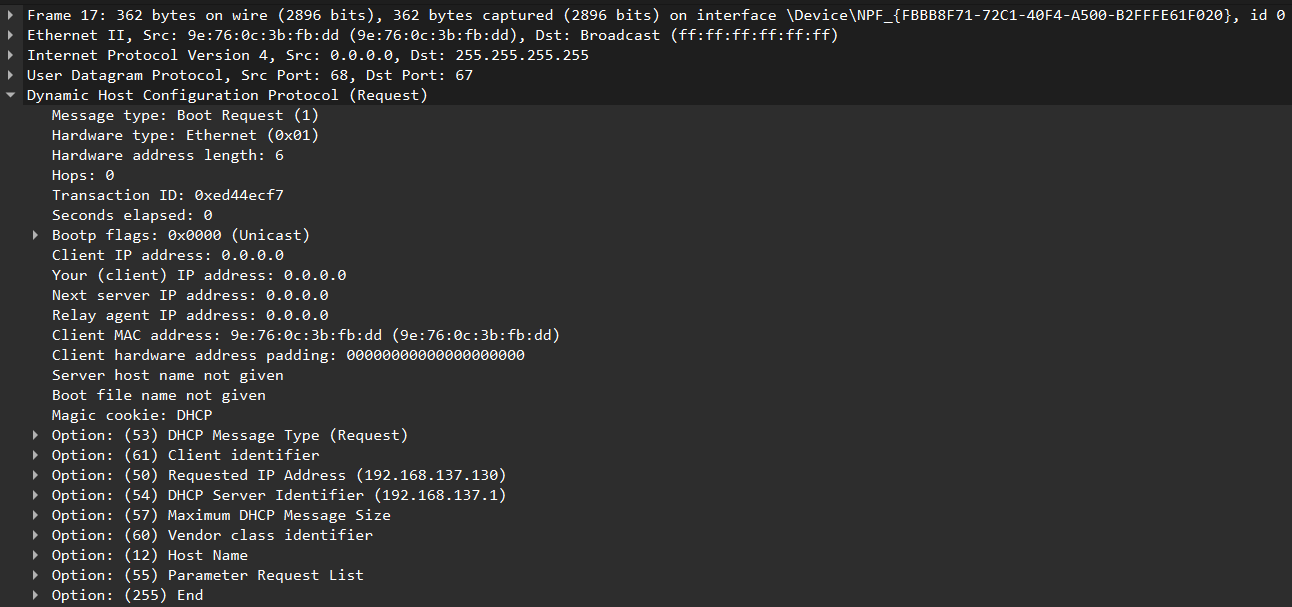
\includegraphics[width=\linewidth, height=0.5\textwidth]{screenshot011}
		\end{minipage}\hfill
		\begin{minipage}{0.49\textwidth}
			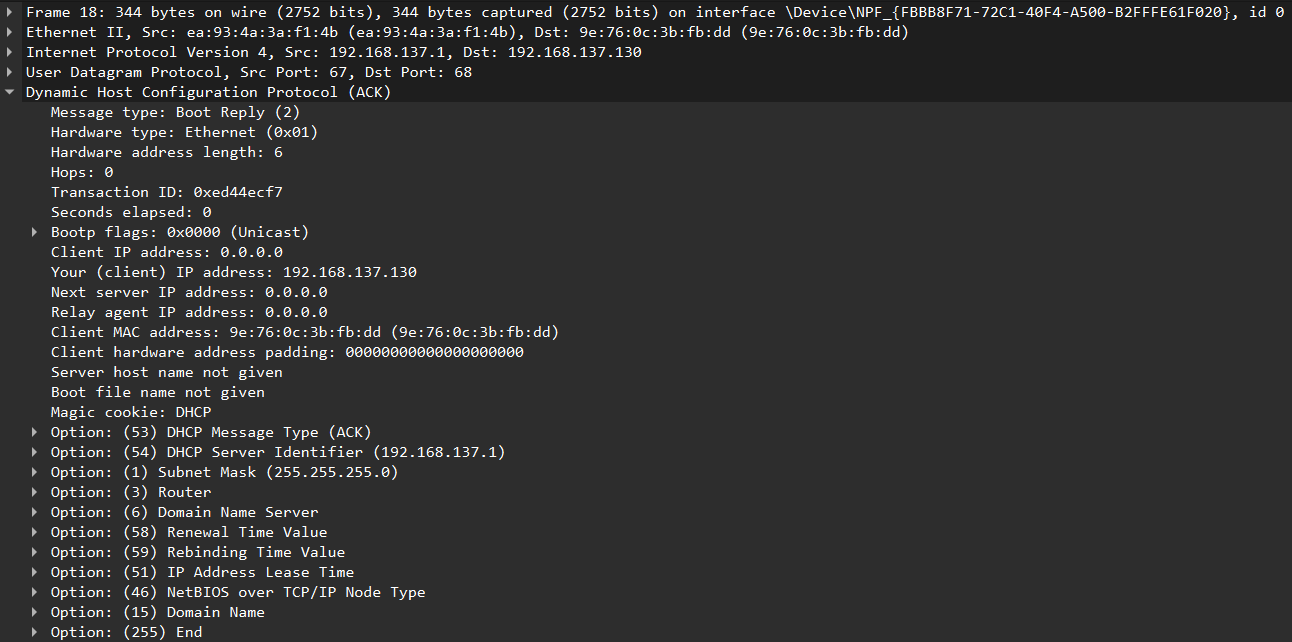
\includegraphics[width=\linewidth]{screenshot012}
		\end{minipage}\hfill
		\caption{DHCP Request and Acknowledgment packet details}
		\label{2}
	\end{figure}
	
	\begin{enumerate}
		\item Which device is the DHCP server in this setup? What is its IP and MAC address?
		
		The DHCP server is my laptop since it's providing hotspot. As observed in the preceding figure, the server IP address is \colorbox{lime}{192.168.137.1} and the server MAC address is \colorbox{lime}{ea:93:4a:3a:f1:4b}.
		
		\item Which device is the DHCP client? What IP address is assigned to it?
		
		The DHCP client is my phone because it is requesting IP. The client IP address and MAC address are \colorbox{lime}{192.168.137.130} and \colorbox{lime}{9e:76:0c:3b:fb:dd} respectively.
		
		\item \textbf{In the DHCP Discover packet:} What is the source MAC address? What is the destination MAC and IP address?
		
		The source MAC address is \colorbox{lime}{9e:76:0c:3b:fb:dd}. The destination MAC and IP addresses are \colorbox{lime}{ff:ff:ff:ff:ff:ff} and \colorbox{lime}{255.255.255.255} respectively because it is broadcast.
		
		\pagebreak
		
		\item \textbf{In the DHCP Offer packet:} What IP address is offered to the phone? What information does the server provide in the DHCP Options (e.g., gateway, DNS)?
		
		The IP address offered and assigned to my phone is \colorbox{lime}{192.168.137.130} . The info provided in the DHCP options are demonstrated in the following figure.
		
		\begin{figure}[!h]
			\centering
			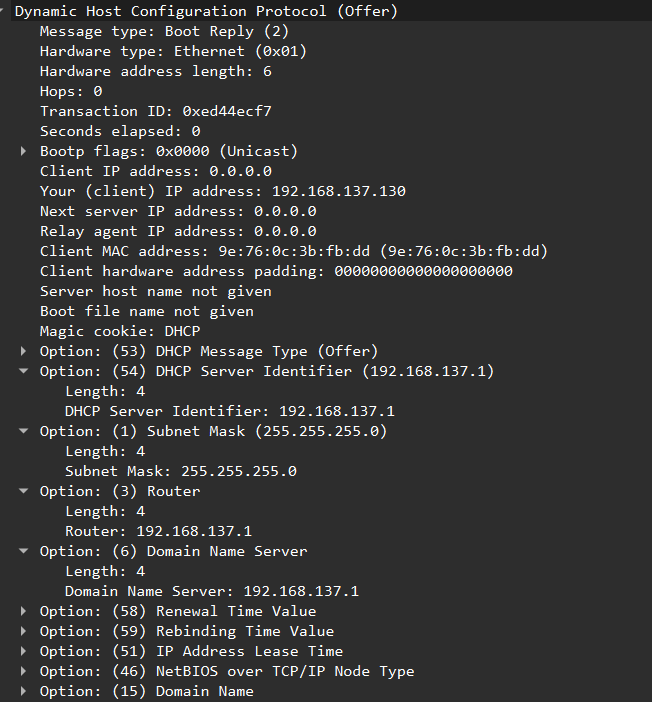
\includegraphics[width=0.6\linewidth]{screenshot014}
			\caption{The provided information in DHCP options of DHCP offer packet}
			\label{fig:screenshot014}
		\end{figure}
		
		The DHCP server provides the router/gateway address as \colorbox{lime}{192.168.137.1}. The DHCP server provides the DNS address as \colorbox{lime}{192.168.137.1}. The subnet mask offered is \colorbox{lime}{255.255.255.0}. Other options are also provided such as lease time, renewal time, and rebind time.
		
		\item What is the role of your laptop in this DHCP exchange? Is it acting like a NAT device too?
		
		My laptop is acting as a DHCP server because it is providing IP address assignments to my phone. It is also functioning as a mobile hotspot to share its network connection with my phone.
		
		Yes, the laptop is acting like a NAT (Network Address Translation) device because it provides internet access to my phone via the mobile hotspot. This process translates the private IP address of the phone (\colorbox{lime}{192.168.137.130}) into the public IP address of my laptop's network interface, enabling my phone to access the internet.
		
		\item Did you observe any difference between this exchange and the one in the earlier wired/wireless DHCP test? Explain
		briefly.
		
		The main difference is in the IP address range. The mobile hotspot assigns IP addresses from the \colorbox{lime}{192.168.137.x} range, while the Wi-Fi interface assigns addresses from the \colorbox{lime}{192.168.100.x} range.
		Also the Wi-Fi interface exchange includes a Requested IP Address in the DHCP Discover message, and the server responds with that specific IP in the Offer packet, while the mobile hotspot just offers a dynamically assigned IP address.
		
	\end{enumerate}
		
		\pagebreak
		
		\subsection{Analyze ARP Protocol}
		
		\subsubsection{Simulation Scenario}
		
		I started capturing packets on the WiFi interface then cleared ARP cache using the command \textit{arp -d *} in the command prompt. After a few seconds I stopped the capture and filtered the ARP packets.
		
		\begin{figure}[!h]
			\centering
			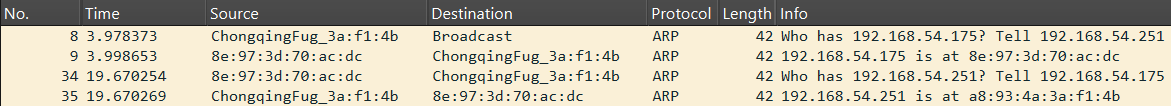
\includegraphics[width=0.7\linewidth]{screenshot015}
			\caption{The filtered arp packets}
			\label{fig:screenshot015}
		\end{figure}
		
		\subsubsection{Questions}
		
		\begin{figure}[!htb]
			\begin{minipage}{0.49\textwidth}
				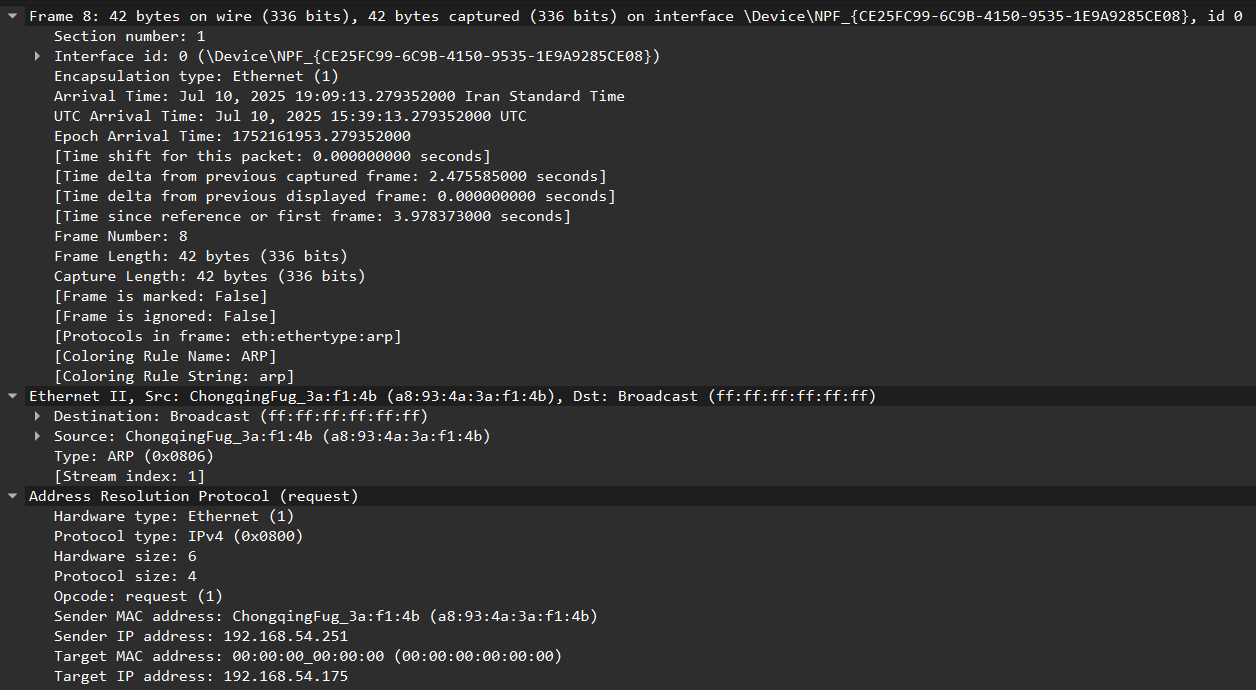
\includegraphics[width=\linewidth]{screenshot016}
			\end{minipage}\hfill
			\begin{minipage}{0.49\textwidth}
				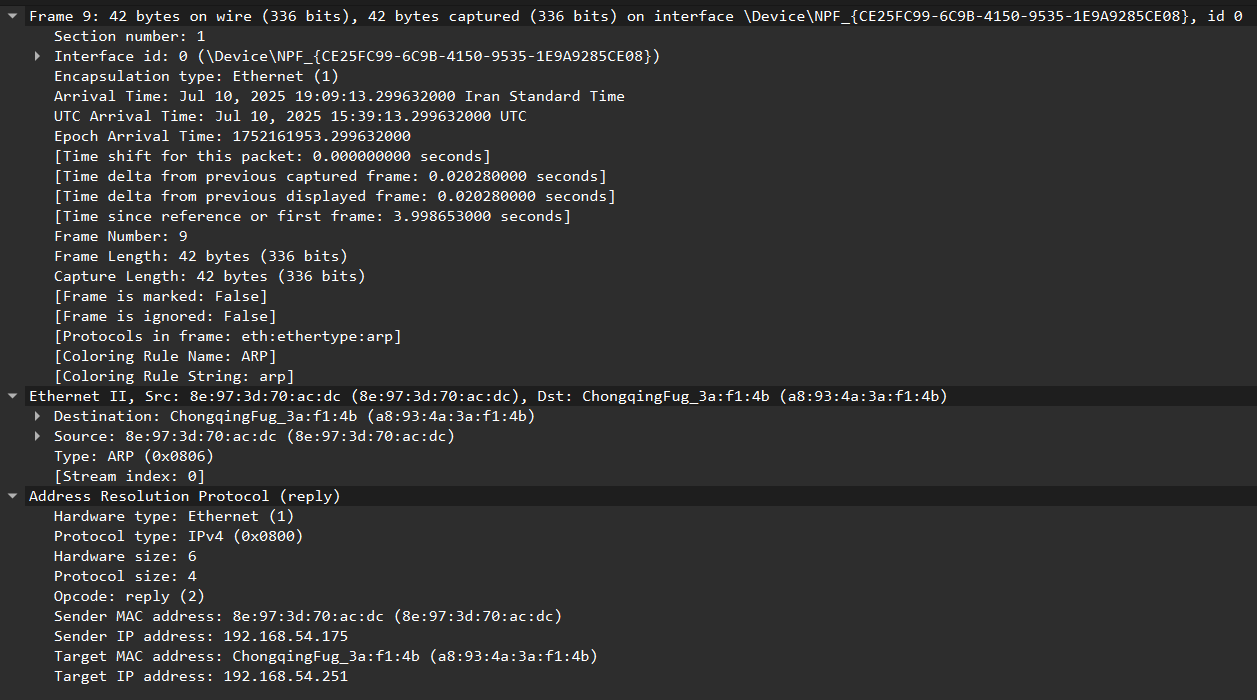
\includegraphics[width=\linewidth]{screenshot017}
			\end{minipage}\hfill
			\caption{The first ARP request and ARP reply packet details}
			\label{1}
		\end{figure}
		\begin{figure}[!htb]
			\begin{minipage}{0.49\textwidth}
				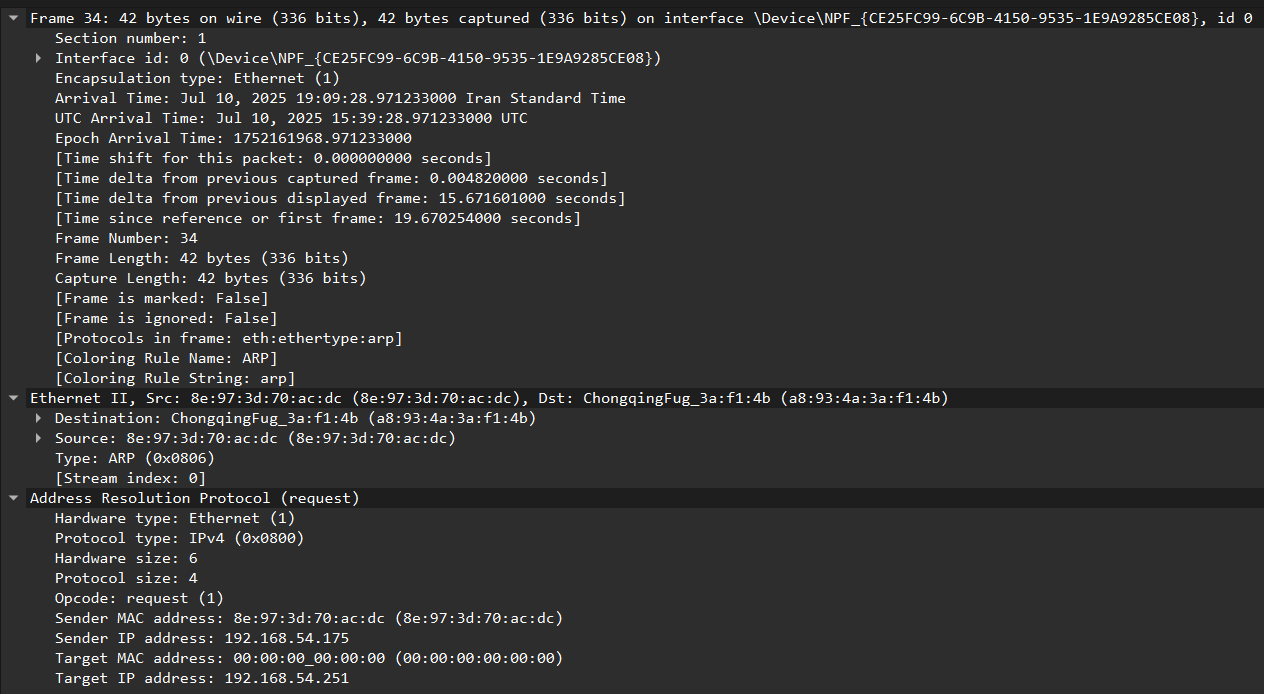
\includegraphics[width=\linewidth]{screenshot018}
			\end{minipage}\hfill
			\begin{minipage}{0.49\textwidth}
				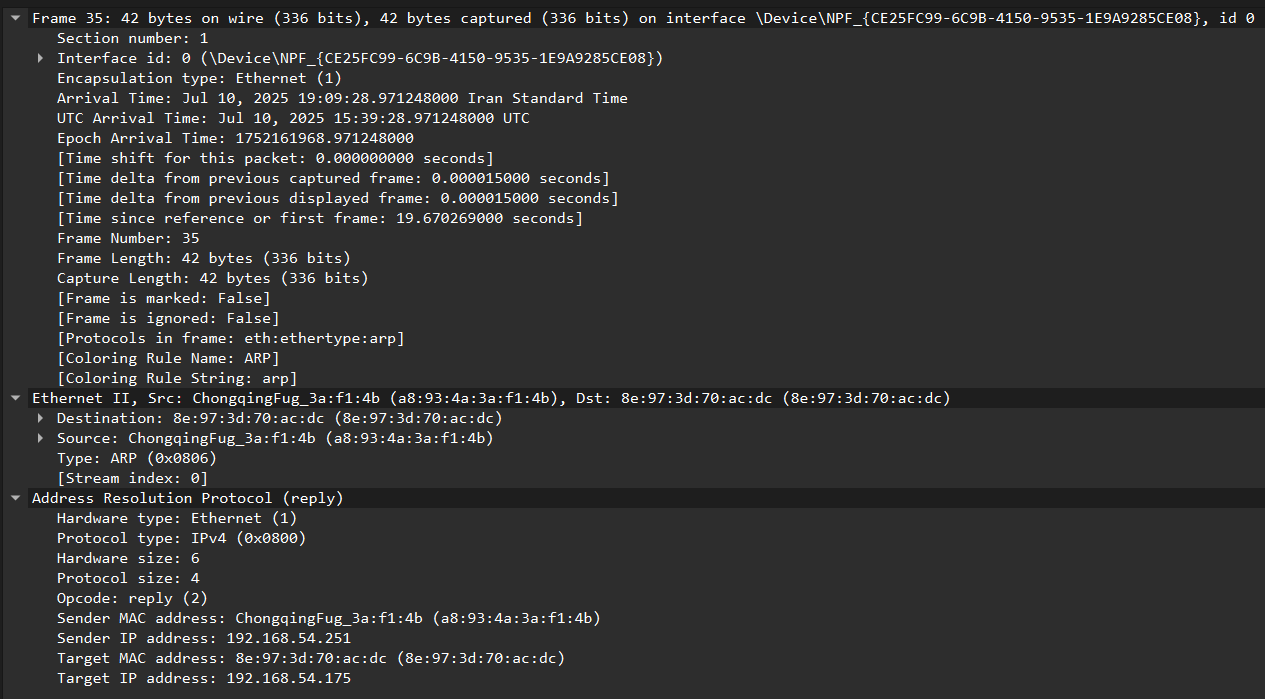
\includegraphics[width=\linewidth]{screenshot019}
			\end{minipage}\hfill
			\caption{The second ARP request and ARP reply packet details}
			\label{2}
		\end{figure}
		
		\begin{enumerate}
			\item Identify the source and destination MAC and IP addresses.
			
			In the first ARP request (frame 8) source (sender) MAC and IP addresses are \colorbox{lime}{a8:93:4a:3a:f1:4b} and \colorbox{lime}{192.168.54.251} and destination (target) MAC and IP addresses are \colorbox{lime}{00:00:00:00:00:00} (broadcast) and \colorbox{lime}{192.168.54.175} respectively.
			
			In the first ARP reply (frame 9) source (sender) MAC and IP addresses are \colorbox{lime}{8e:97:3d:70:ac:dc} and \colorbox{lime}{192.168.54.175} and destination (target) MAC and IP addresses are \colorbox{lime}{a8:93:4a:3a:f1:4b} and \colorbox{lime}{192.168.54.251} respectively.
			
			In the second ARP request (frame 34) source (sender) MAC and IP addresses are \colorbox{lime}{8e:97:3d:70:ac:dc} and \colorbox{lime}{192.168.54.175} and destination (target) MAC and IP addresses are \colorbox{lime}{00:00:00:00:00:00} (broadcast) and \colorbox{lime}{192.168.54.251} respectively.
			
			In the second ARP reply (frame 35) source (sender) MAC and IP addresses are \colorbox{lime}{a8:93:4a:3a:f1:4b} and \colorbox{lime}{192.168.54.251} and destination (target) MAC and IP addresses are \colorbox{lime}{8e:97:3d:70:ac:dc} and \colorbox{lime}{192.168.54.175} respectively.
			
			\pagebreak
			
			\item Explain the packet’s purpose (e.g., ARP request or reply).
			
			The ARP request is sent by a device when it needs to find the MAC address corresponding to an IP address on the local network.
			
			The ARP reply is sent by the device that has the requested IP address, responding with its MAC address.
			
			\item Open the ARP section in the Packet Details window and describe its fields.
			
			\begin{itemize}
				\item Hardware type:
				
					Ethernet (1), meaning the ARP is for resolving Ethernet MAC addresses.
					
				\item Protocol type:
					
					IPv4 (0x0800), indicating that this ARP request/reply is related to IPv4.
					
				\item Hardware size:
				
					6, which is the size of the MAC address (6 bytes).
					
				\item Protocol size:
				
					4, which is the size of the IP address (4 bytes).
					
				\item Opcode:
				
					1 for ARP request and 2 for ARP reply. The ARP request asks "Who has this IP?" while the ARP reply answers with the MAC address.
					
				\item Sender MAC address:
					
					The MAC address of the device sending the ARP message.
					
				\item Sender IP address:
				
					The IP address of the device sending the ARP message.
					
				\item Target MAC address:
					
					The MAC address of the device being queried.
					
				\item Target IP address:
				
					The IP address of the device being queried.
			
			\end{itemize}
			
			\item Why does the system need to use ARP before sending the first ping packet?
			
			The system needs to use ARP (Address Resolution Protocol) before sending a ping because ARP is necessary to resolve the MAC address associated with the destination IP address in the local network.
			
			A ping packet requires the MAC address of the destination device to be able to send the data link (Ethernet) frame.
			
			\item Are ARP messages sent as broadcast or unicast? How can you tell from the packet capture?
			
			ARP requests are broadcasted because the sender does not know which device has the requested IP address.
			
			ARP replies are unicasted to the device that requested the information.
			
		\end{enumerate}
		
		\subsection{Analyze NAT Behavior Using Wireshark}
		
		\subsubsection{Simulation Scenario}
		
			I captured packets using two instances of WireShark and then filtered the captured packets after the speed test process was over. Then I saved the selected packets in two .pcapng files named WiFi and HotSpot.
		
		\pagebreak
		
		\subsubsection{Questions}
		
		\begin{enumerate}
			\item What is the IP address of your phone in the hotspot capture? What port did it use to initiate the connection?
			
			\begin{figure}[!h]
				\centering
				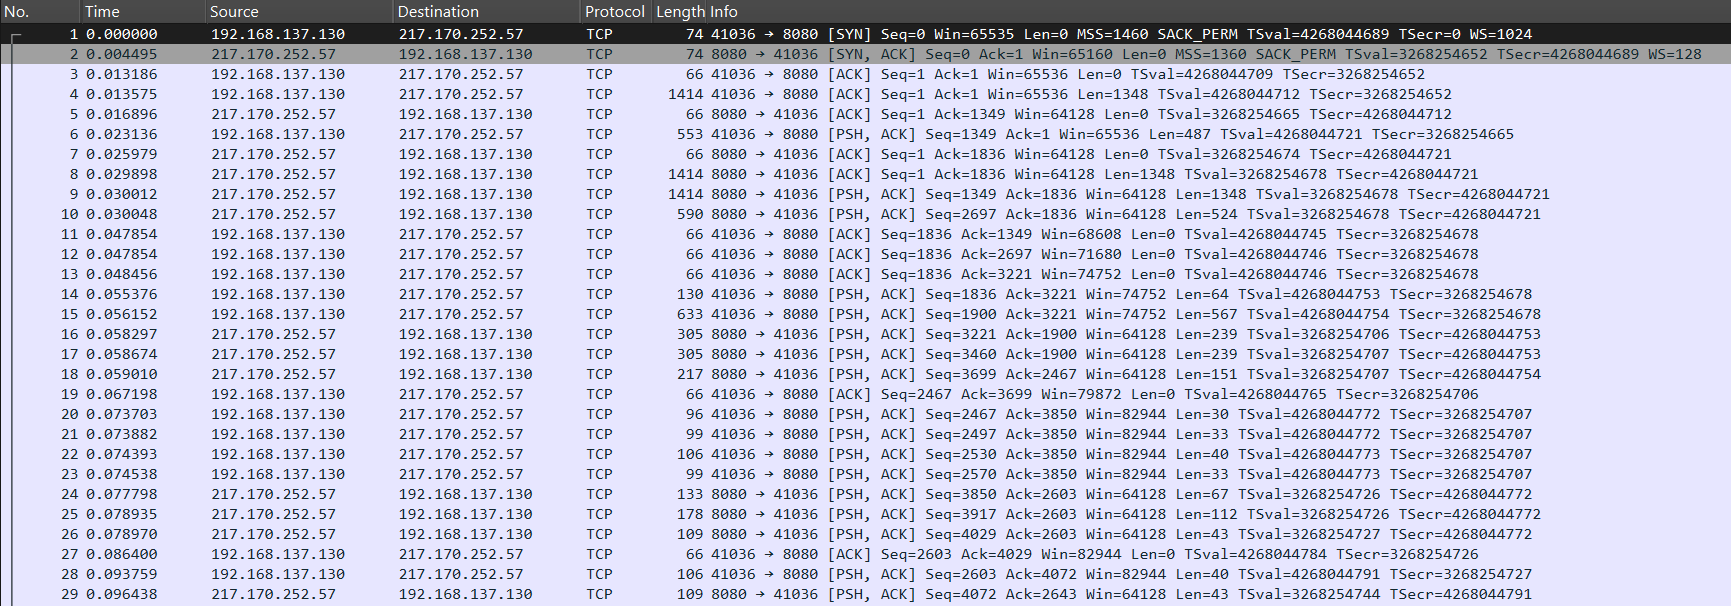
\includegraphics[width=0.7\linewidth]{screenshot071}
				\caption{The first few filtered packets in the HotSpot capture}
				\label{fig:screenshot071}
			\end{figure}
			
			According to the first packet the IP address of my phone in the hotspot capture is \colorbox{lime}{192.168.137.130} . The source port used to initiate the connection was 41036 based of the info section of the first packet presented in \ref{fig:screenshot071}.
			
			\item What is the destination IP and port (i.e., the server performing the speed test)?
			
			\begin{figure}[!h]
				\centering
				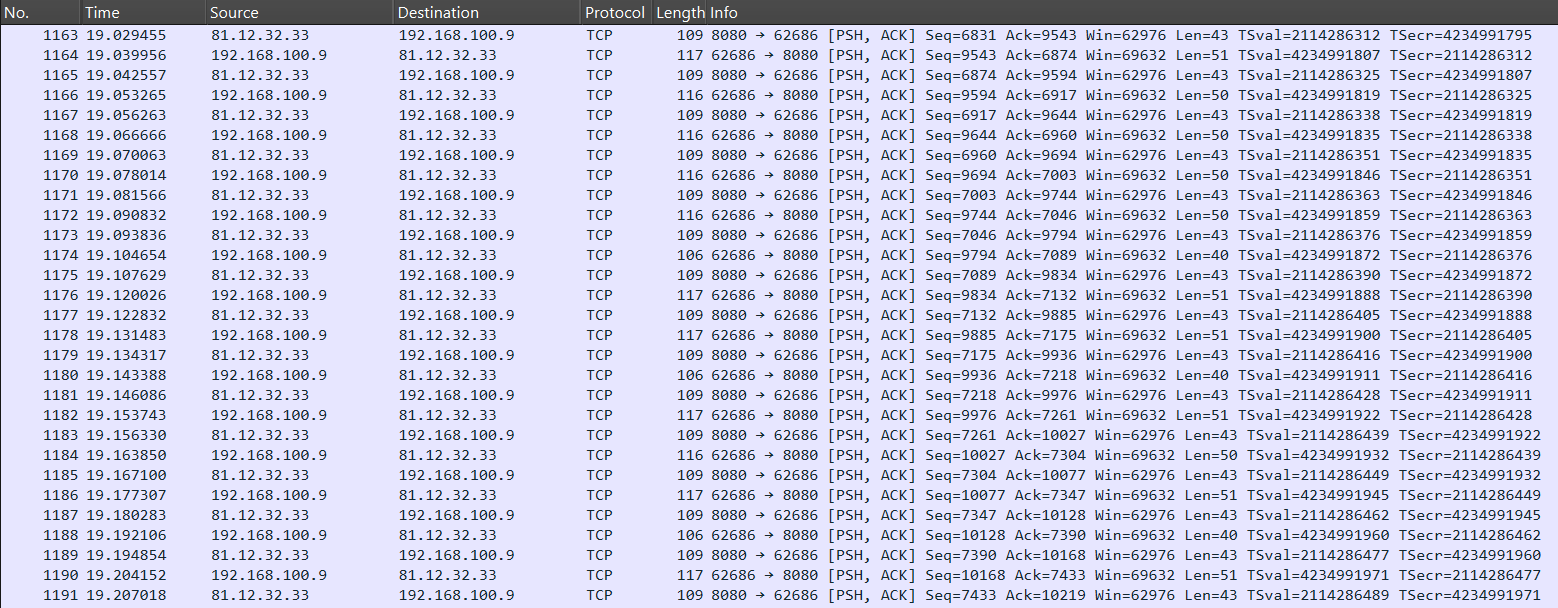
\includegraphics[width=0.7\linewidth]{screenshot072}
				\caption{Some test packets in WiFi capture}
				\label{fig:screenshot072}
			\end{figure}
			\begin{figure}[!h]
				\centering
				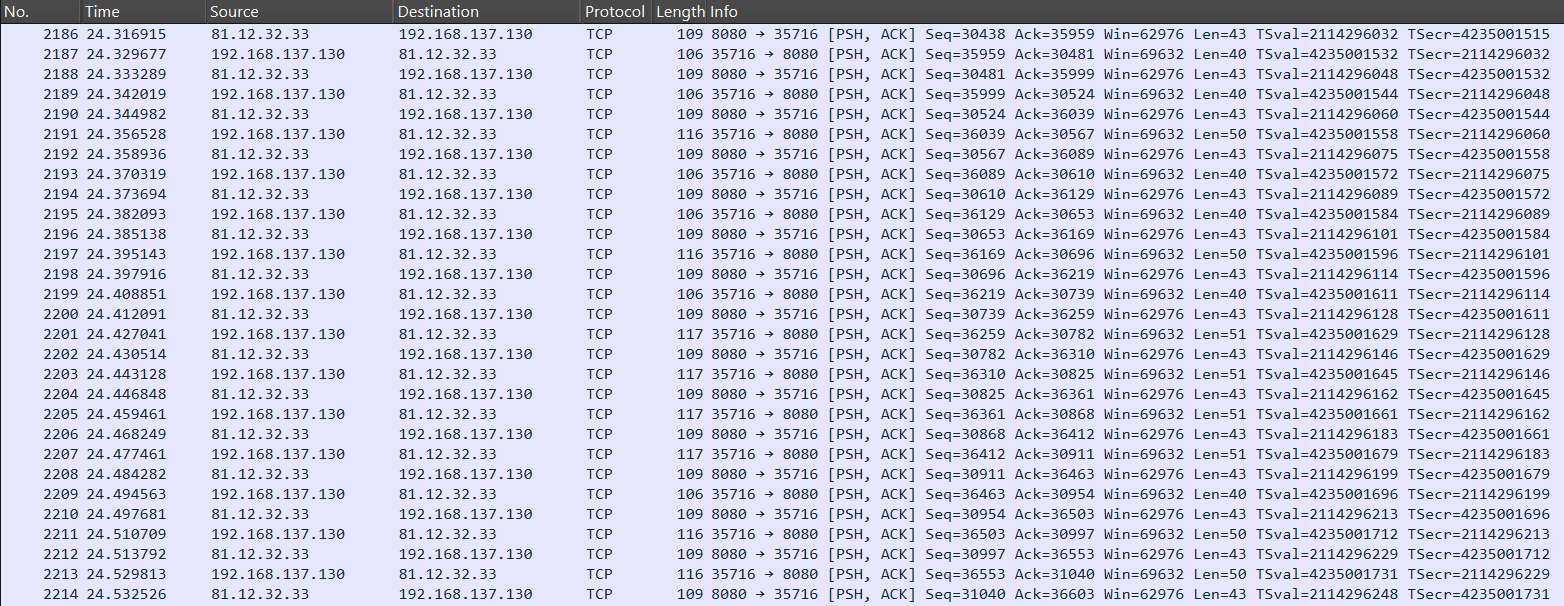
\includegraphics[width=0.7\linewidth]{screenshot073}
				\caption{Some test packets in HotSpot capture}
				\label{fig:screenshot073}
			\end{figure}
			
			Based on the figures presented above, the IP address of the server performing the speed test is \colorbox{lime}{81.12.32.33}. The destination port is 8080.
			
			\item Compare the IP addresses and ports in both captures. Explain how NAT translated them.
			
			HotSpot capture:
			
			phone IP: \colorbox{lime}{192.168.137.130} \qquad phone Port: 41036 \\
			server IP: \colorbox{lime}{81.12.32.33} \quad\quad\quad\quad server Port: 8080 \\
			
			WiFi Capture:
			
			phone IP: \colorbox{lime}{192.168.100.9} \quad\qquad phone Port: 62532 \\
			server IP: \colorbox{lime}{81.12.32.33} \quad\quad\quad\quad server Port: 8080 \\
			
			NAT translated my phone’s private IP and port \colorbox{lime}{192.168.137.130:41036} into my laptop’s IP and a new port \colorbox{lime}{192.168.100.9:62532} to enable internet access. Since private IPs aren't routable on the internet, the laptop changed the source address and kept a mapping in its NAT table. When the server responded, NAT reversed the translation and delivered the reply back to the phone, ensuring proper communication between the device and the server.
			
			\item Why is NAT needed in this case? Could your phone directly access the internet without the translation?
			
			NAT is essential in this scenario because the phone’s private IP is not routable on the public internet, and the laptop must act as a gateway to translate the phone’s traffic.\\
			Without NAT, my phone could not communicate with the speed test server, as its private IP would prevent proper routing and response handling.
			
			
			
		\end{enumerate}
		
		
		
		
		\subsection{Analyze Traceroute Using ICMP}
		
		\subsubsection{Simulation Scenario}
		
		I started capturing traffic on the WiFi interface and then ran the traceroute command \textit{tracert 8.8.8.8} to Google DNS. After a few seconds the traceroute completed and I stopped the capture. The filtered ICMP packets are demonstrated in the following figures.
		
		\begin{figure}[!h]
			\centering
			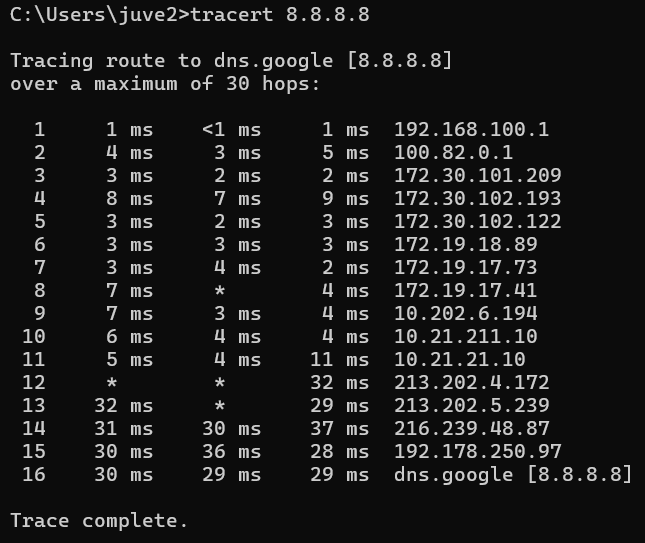
\includegraphics[width=0.6\linewidth]{screenshot024}
			\caption{Traceroute to Google result}
			\label{fig:screenshot024}
		\end{figure}
		
		\begin{figure}[!htb]
			\begin{minipage}{0.49\textwidth}
				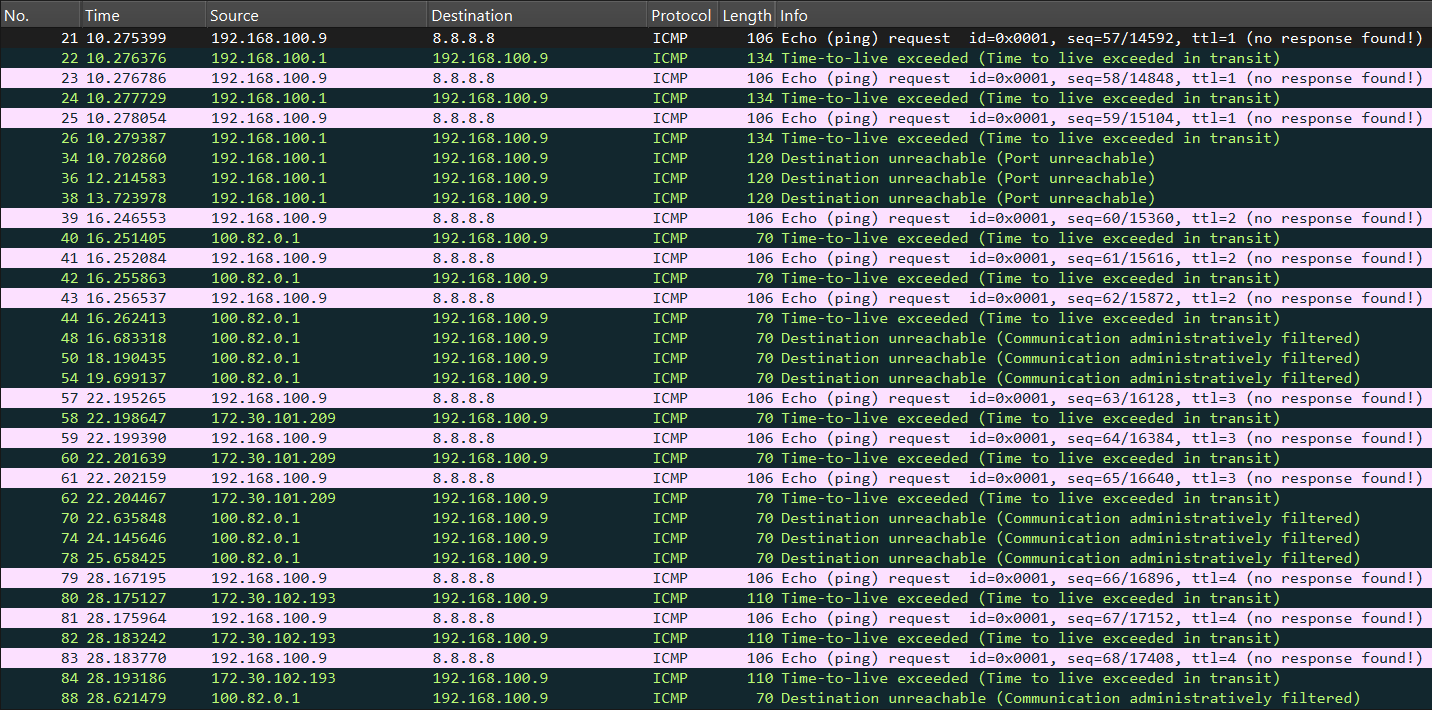
\includegraphics[width=\linewidth]{screenshot020}
			\end{minipage}\hfill
			\begin{minipage}{0.49\textwidth}
				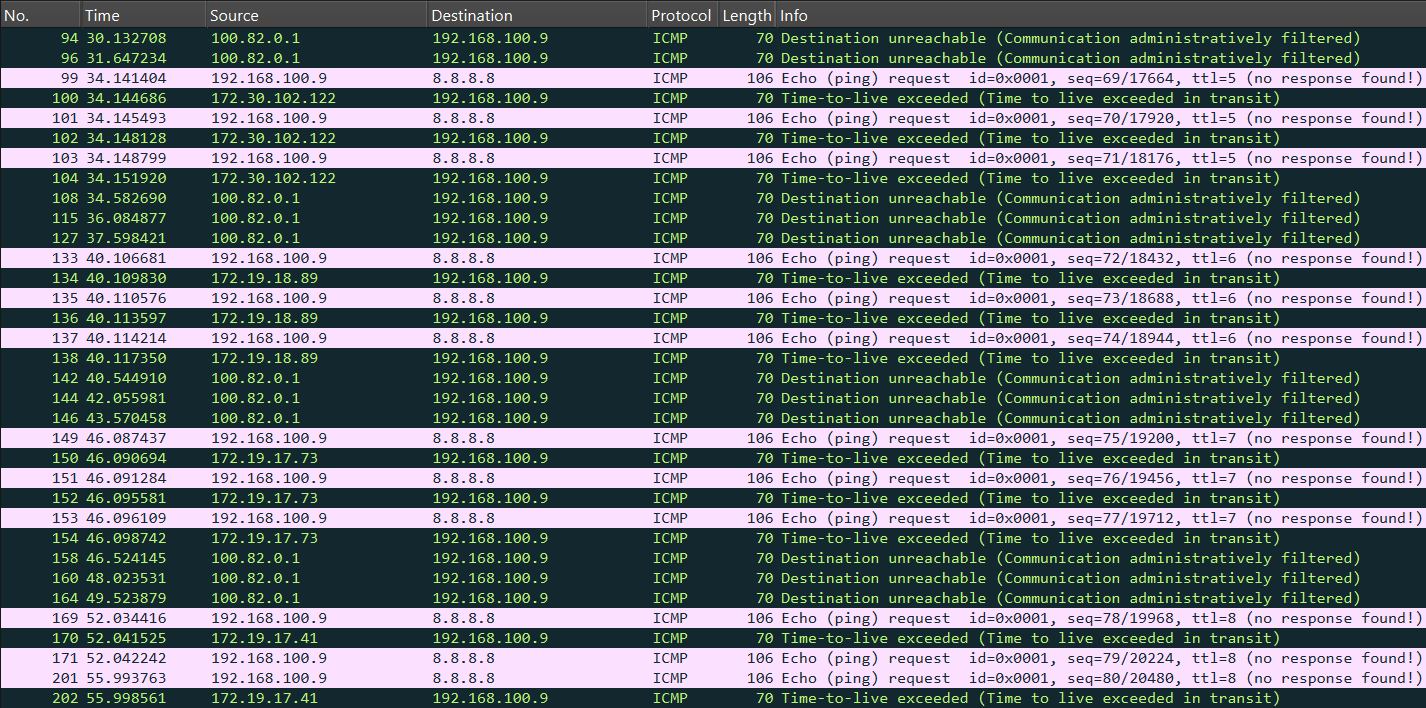
\includegraphics[width=\linewidth]{screenshot021}
			\end{minipage}\hfill
			\caption{The ICMP packets}
			\label{1}
		\end{figure}
		\begin{figure}[!htb]
			\begin{minipage}{0.49\textwidth}
				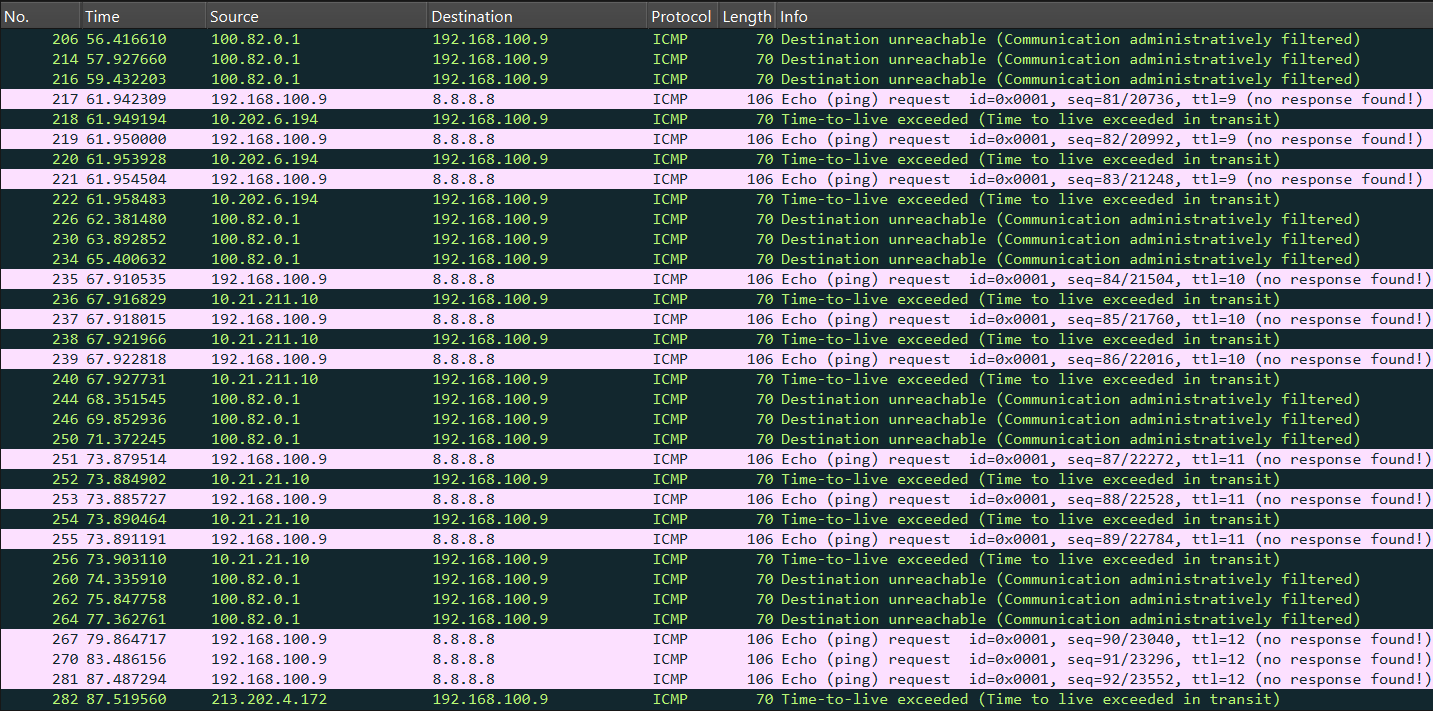
\includegraphics[width=\linewidth]{screenshot022}
			\end{minipage}\hfill
			\begin{minipage}{0.49\textwidth}
				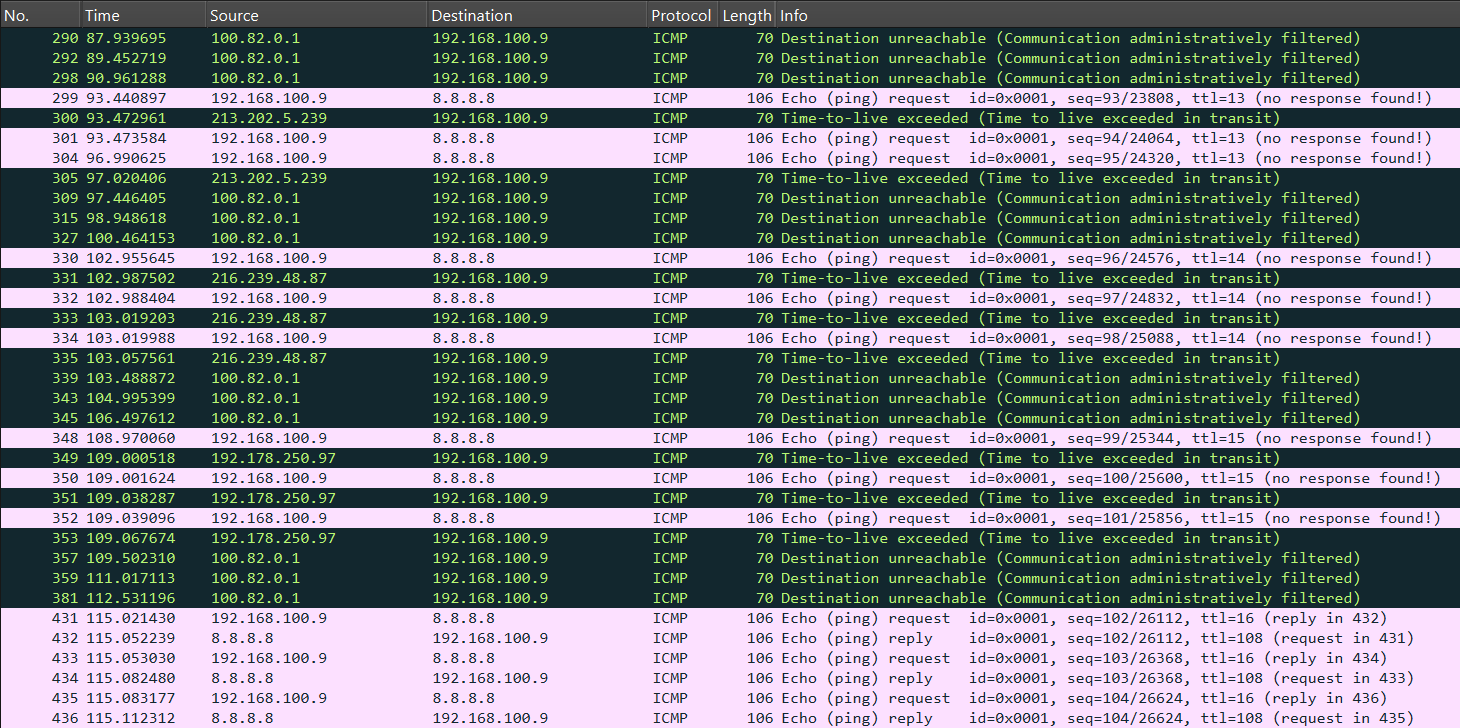
\includegraphics[width=\linewidth]{screenshot023}
			\end{minipage}\hfill
			\caption{The ICMP packets}
			\label{2}
		\end{figure}
		
		\pagebreak
		
		\subsubsection{Questions}
		
		\begin{enumerate}
			\item How many hops did it take to reach 8.8.8.8? List the IP addresses of any 3 hops.
			
			According to the figures in the previous page, the total number of hops took to reach the destination was 16 hops.
			
			The hops respectively:
			\begin{center}
				192.168.100.9$\longrightarrow$
				192.168.100.1$\longrightarrow$
				100.82.0.1$\longrightarrow$
				172.30.101.209$\longrightarrow$
				172.30.102.193$\longrightarrow$
				172.30.102.122$\longrightarrow$
				172.19.18.89$\longrightarrow$
				172.19.17.73$\longrightarrow$
				172.19.17.41$\longrightarrow$
				10.202.6.194$\longrightarrow$
				10.21.211.10$\longrightarrow$
				10.21.21.10$\longrightarrow$
				213.202.5.239$\longrightarrow$
				216.239.48.87$\longrightarrow$
				192.178.250.97$\longrightarrow$
				8.8.8.8
			\end{center}
			
			\item What type of ICMP messages were generated by intermediate routers?
			
			The ICMP message type generated by intermediate routers is Time to live exceeded (Type 11 Code 0).
			
			These time exceeded messages are generated when the Time to Live (TTL) of a packet reaches zero before it reaches its destination. This shows that the packet has been forwarded through multiple routers but has not yet reached the destination.
			
			\item Pick one Time Exceeded packet and describe its source IP, destination IP, and TTL value in the IP header.
			
			\begin{figure}[!h]
				\centering
				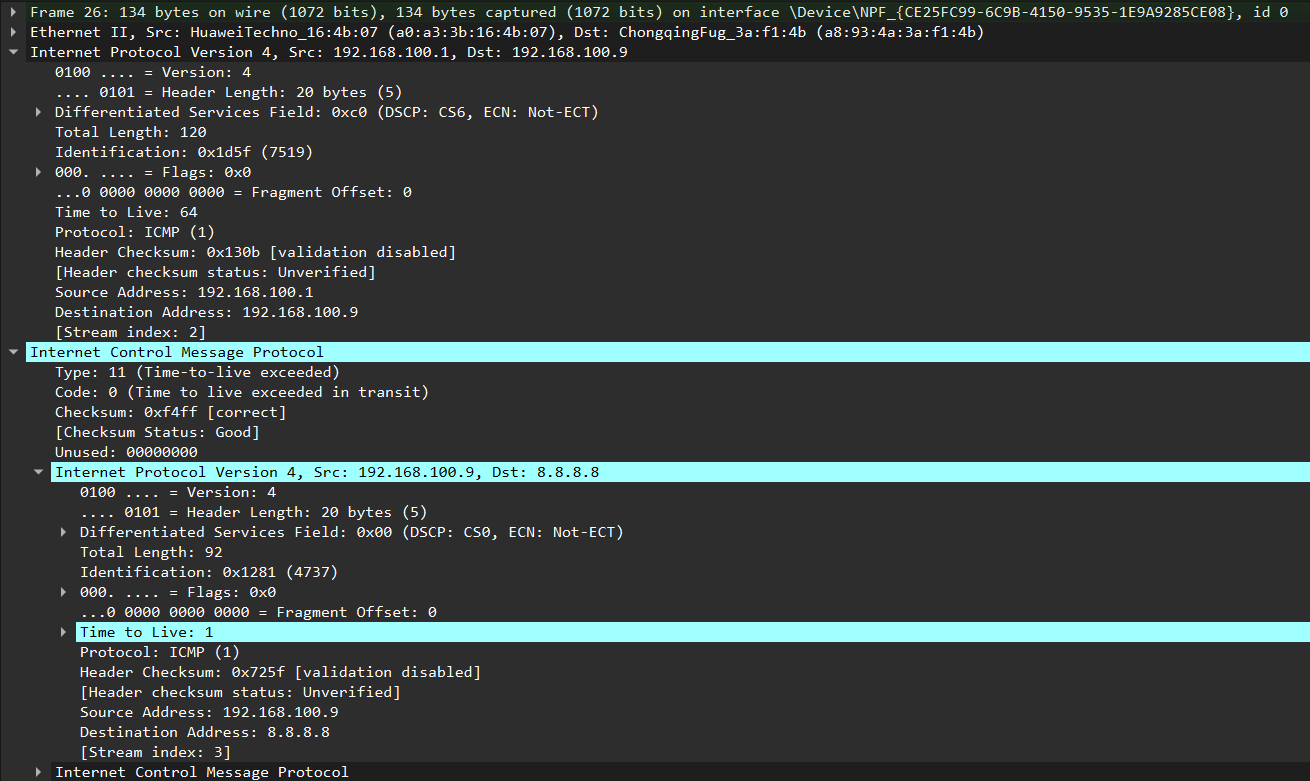
\includegraphics[width=0.7\linewidth]{screenshot025}
				\caption{The details of the first Time Exceeded packet}
				\label{fig:screenshot025}
			\end{figure}
			
			According to this figure,
			
			Source IP address: \colorbox{lime}{192.168.100.1}
			
			Destination IP address: \colorbox{lime}{192.168.100.9}
			
			TTL: 64
			
			\item Why do intermediate routers generate Time Exceeded messages?
			
			If the TTL reaches zero before the packet reaches the destination, the router sends an ICMP Time Exceeded message back to the source, notifying that the packet was discarded due to TTL expiration.
			
			This mechanism is used to track the path a packet takes across the network by setting the TTL value and receiving ICMP responses from each router.
			
			\item What happens to the TTL value in each step of the traceroute?
			
			TTL starts from a low value (here 1) and increases with each subsequent packet.
			
			In the first hop the TTL is set to 1, so the first router will discard the packet, sending back an ICMP Time Exceeded message.
			
			In the next hop TTL is incremented to 2, allowing the packet to reach the second router, which decreases the TTL to 1. This router then responds with a Time Exceeded message.
			
			This process continues, increasing the TTL by 1 each time until the packet eventually reaches the destination or the maximum number of hops is reached(here 30).
			
			\item Is the final destination’s response different from the intermediate hops? What ICMP type/code does it return?
			
			Yes the final destination's response is an Echo reply with Type 0 and Code 0.
			
			\begin{figure}[h!]
				\centering
				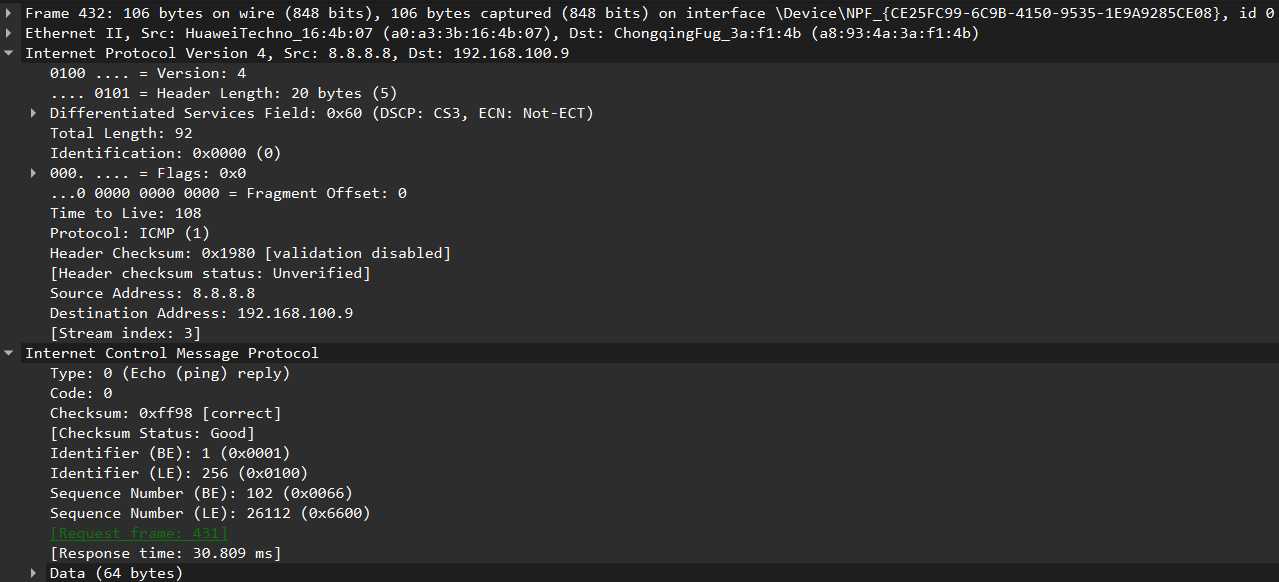
\includegraphics[width=0.7\linewidth]{screenshot026}
				\caption{The final destination response packet details}
				\label{fig:screenshot026}
			\end{figure}
			
			
		\end{enumerate}
		
		\subsection{Analyze IP Fragmentation}
		
		\subsubsection{Simulation Scenario}
		
		\begin{figure}[!h]
			\centering
			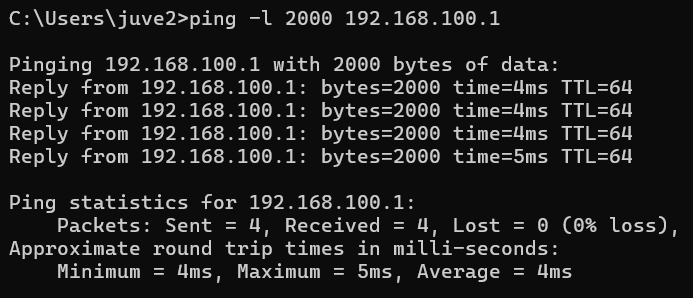
\includegraphics[width=0.7\linewidth]{screenshot028}
			\caption{Ping request result in CMD}
			\label{fig:screenshot028}
		\end{figure}
		
		\begin{figure}[!h]
			\centering
			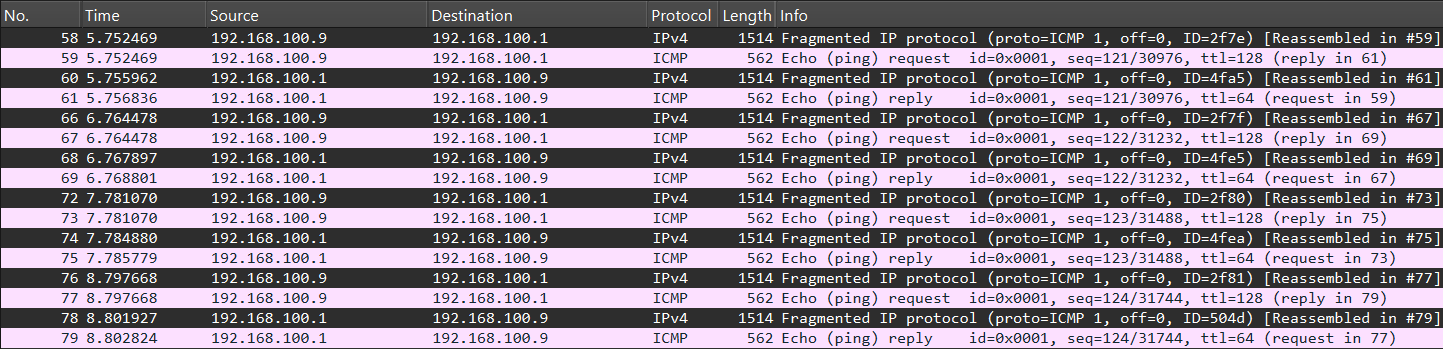
\includegraphics[width=0.7\linewidth]{screenshot027}
			\caption{The filtered packets}
			\label{fig:screenshot027}
		\end{figure}
		
		
		\subsubsection{Questions}
		
		\begin{enumerate}
			\item How many fragments were generated for one large ping request?
			
			As we can see each large ping request is fragmented into two fragments.
			
			\pagebreak
			
			\begin{figure}[!htb]
				\begin{minipage}{0.49\textwidth}
					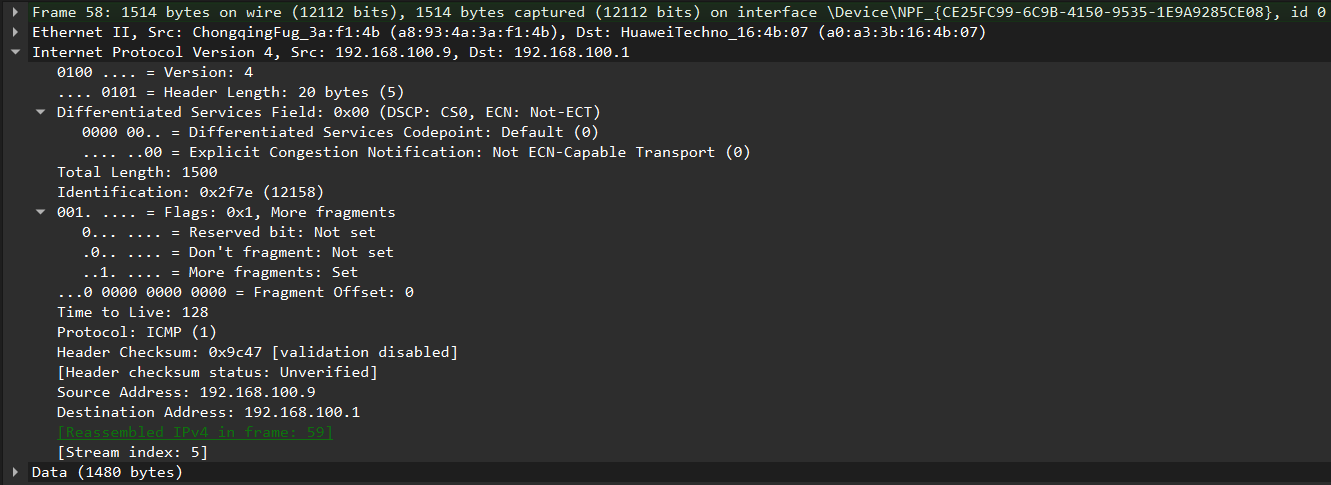
\includegraphics[width=\linewidth, height=0.45\linewidth]{screenshot029}
				\end{minipage}\hfill
				\begin{minipage}{0.49\textwidth}
					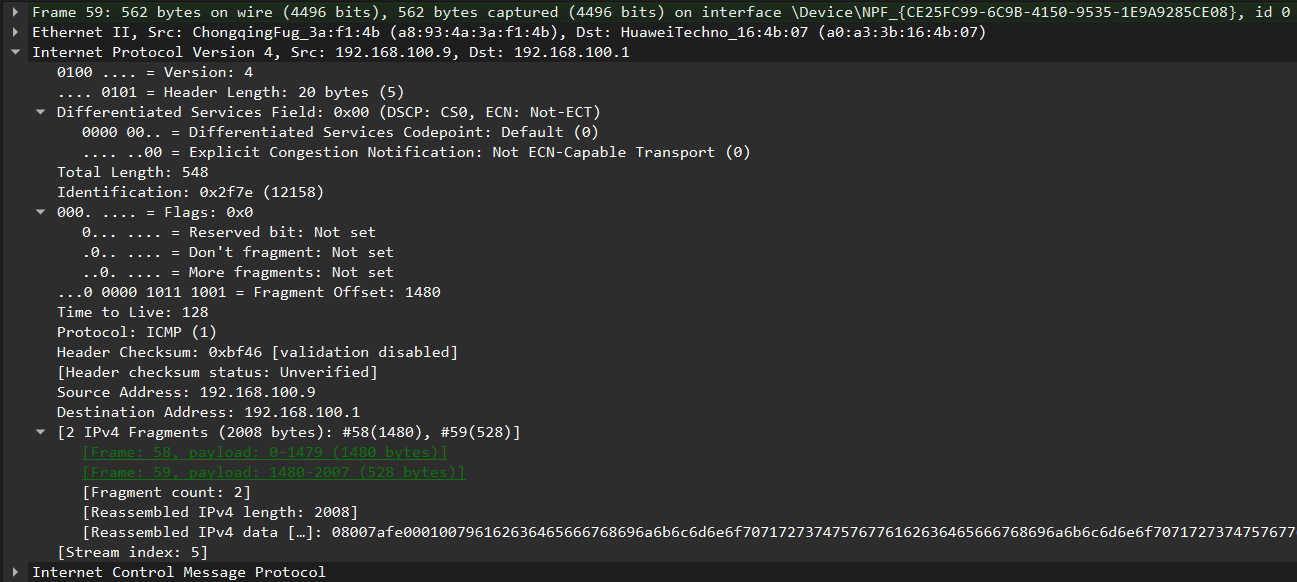
\includegraphics[width=\linewidth, height=0.45\linewidth]{screenshot030}
				\end{minipage}\hfill
				\caption{The two fragments of the first large ping request}
				\label{11}
			\end{figure}
			
			\item What is the total length of each fragment? What is the offset of each?
			
			As observed above, the total length of the first fragment is 1500 bytes and the second fragment 548 bytes.
			
			offset of the first fragment is 0 and the second fragment 1480.
			
			\item What values in the IP header indicate that a packet is fragmented?
			
			The flag in the first fragment is set to 0x1 which means that MF is set and the packet is fragmented and more fragments are expected. The offset in the second fragment is a number greater than 0 (1480) which also indicated that the packet is fragmented.
			
			\item What is the role of the "More Fragments" (MF) flag and Fragment Offset?
			
			The MF flag is used to indicate if the fragment is the last one. If MF = 1, it means there are more fragments to come. If MF = 0, it signifies that this is the last fragment in the packet.
			
			The fragment offset tells the receiving system where the current fragment belongs in the reassembly of the original datagram. It is measured in bytes, so an offset of 1480 means the fragment starts 1480 bytes into the original message.
			
			\item If one fragment is lost during transmission, will the full datagram be delivered?
			
			No.
			If one fragment is lost, the receiving device cannot reassemble the full datagram because it is missing a part of the data. The destination device will normally request the missing fragment or drop the entire datagram if it is incomplete.
			
			\item What is the Identification field used for in fragmented IP packets?
			
			The Identification field is used to group fragments that belong to the same original datagram.
			
			As we can see in \ref{11} both fragments have the Identification 0x2f7e.
			
			\item Are fragmented packets reassembled by routers or by the destination device? Explain briefly.
			
			Reassembly of fragmented packets is done by the destination device.
			
			Routers do not reassemble fragmented packets; they only forward the fragments to the destination.
			
			The destination device uses the Identification field and Fragment Offset to reassemble the fragments into the original datagram.
			
		\end{enumerate}
		
		\subsubsection{Simulation Scenario}
		
		I repeated the previous scenario for DNS servers \colorbox{lime}{8.8.8.8} and \colorbox{lime}{1.1.1.1} . The results are demonstrated in the following figures.
		
		
		\begin{center}
			\Large
			8.8.8.8
		\end{center}
		
		\begin{figure}[!h]
			\centering
			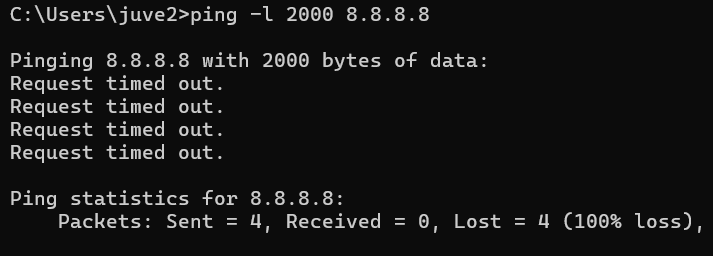
\includegraphics[width=0.7\linewidth]{screenshot034}
			\caption{Ping request result in CMD}
			\label{fig:screenshot034}
		\end{figure}
		\begin{figure}[!h]
			\centering
			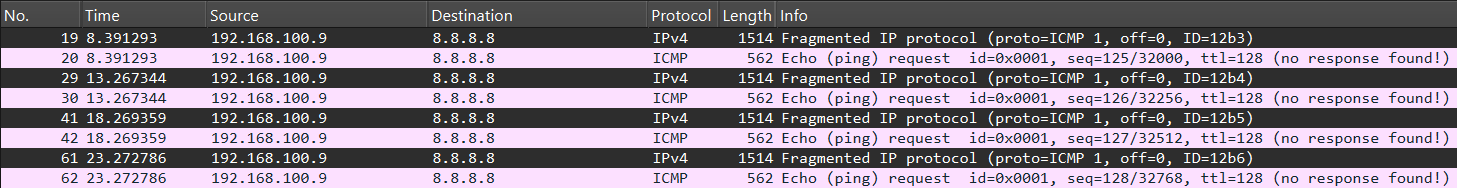
\includegraphics[width=0.7\linewidth]{screenshot031}
			\caption{The filtered packets}
			\label{fig:screenshot031}
		\end{figure}
		
		\begin{figure}[!htb]
			\begin{minipage}{0.49\textwidth}
				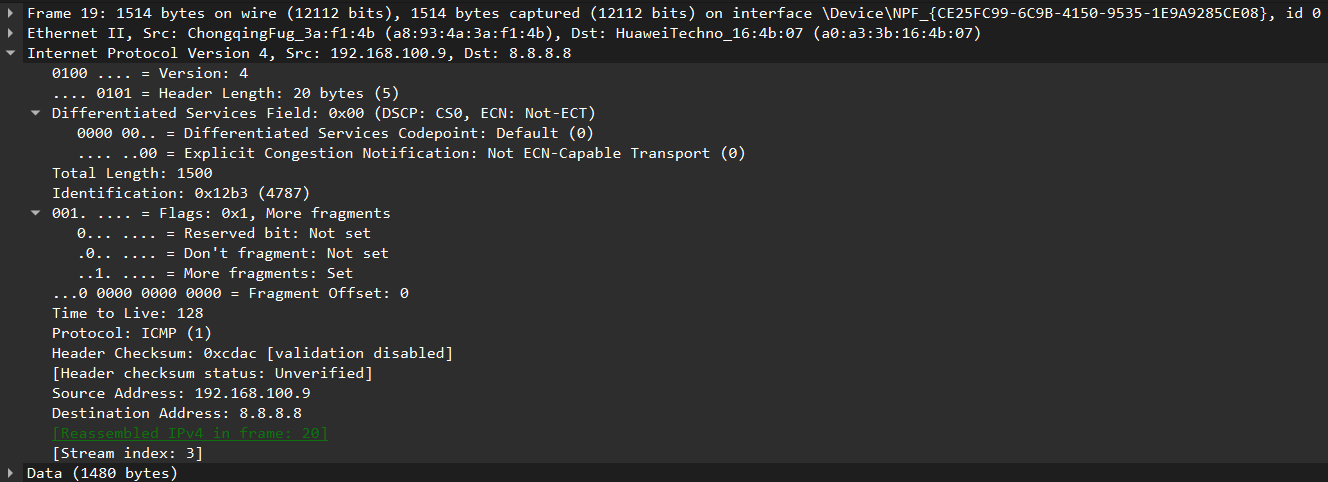
\includegraphics[width=\linewidth, height=0.45\linewidth]{screenshot032}
			\end{minipage}\hfill
			\begin{minipage}{0.49\textwidth}
				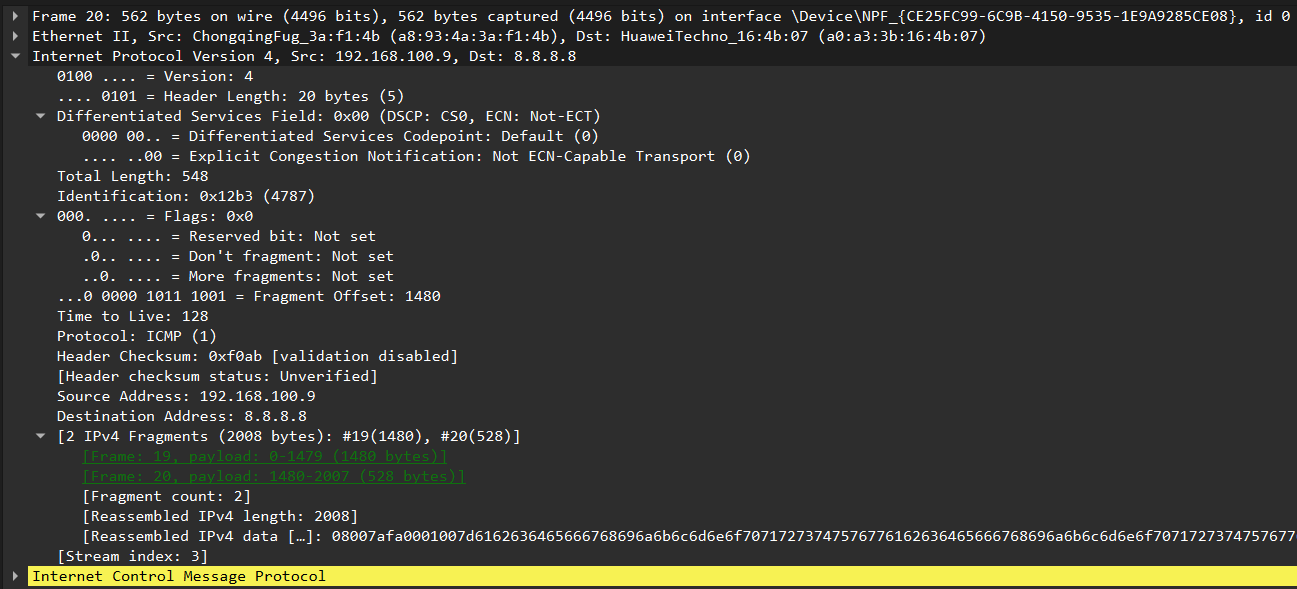
\includegraphics[width=\linewidth, height=0.45\linewidth]{screenshot033}
			\end{minipage}\hfill
			\caption{The two fragments of the first large ping request}
			\label{11}
		\end{figure}
		
		\pagebreak
		
		\begin{center}
			\Large
			1.1.1.1
		\end{center}
		
		\begin{figure}[!h]
			\centering
			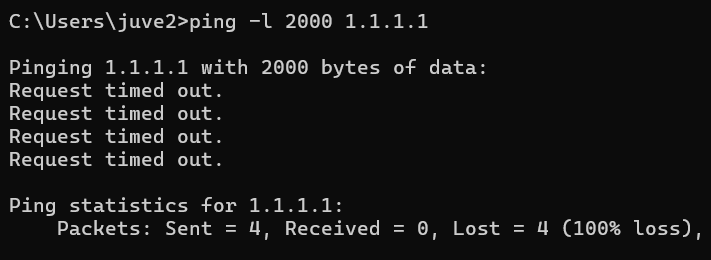
\includegraphics[width=0.7\linewidth]{screenshot035}
			\caption{Ping request result in CMD}
			\label{fig:screenshot035}
		\end{figure}
		\begin{figure}[!h]
			\centering
			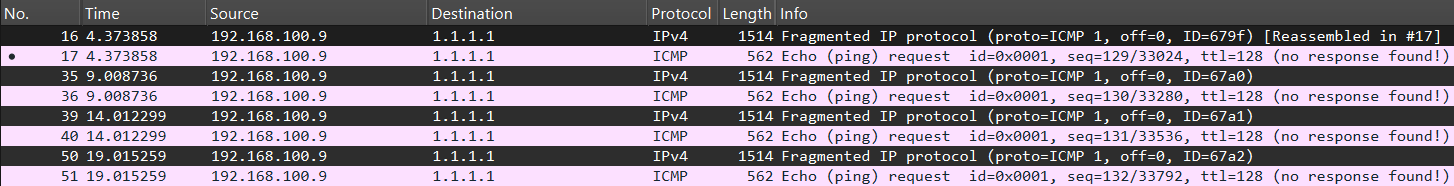
\includegraphics[width=0.7\linewidth]{screenshot036}
			\caption{The filtered packets}
			\label{fig:screenshot036}
		\end{figure}
		
		\begin{figure}[!htb]
			\begin{minipage}{0.49\textwidth}
				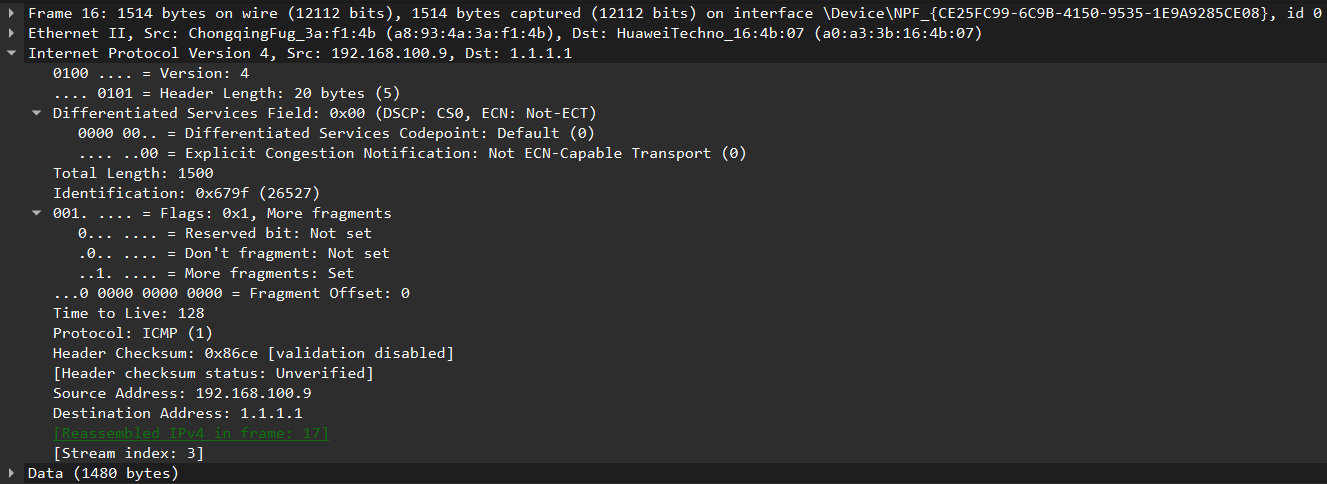
\includegraphics[width=\linewidth, height=0.45\linewidth]{screenshot037}
			\end{minipage}\hfill
			\begin{minipage}{0.49\textwidth}
				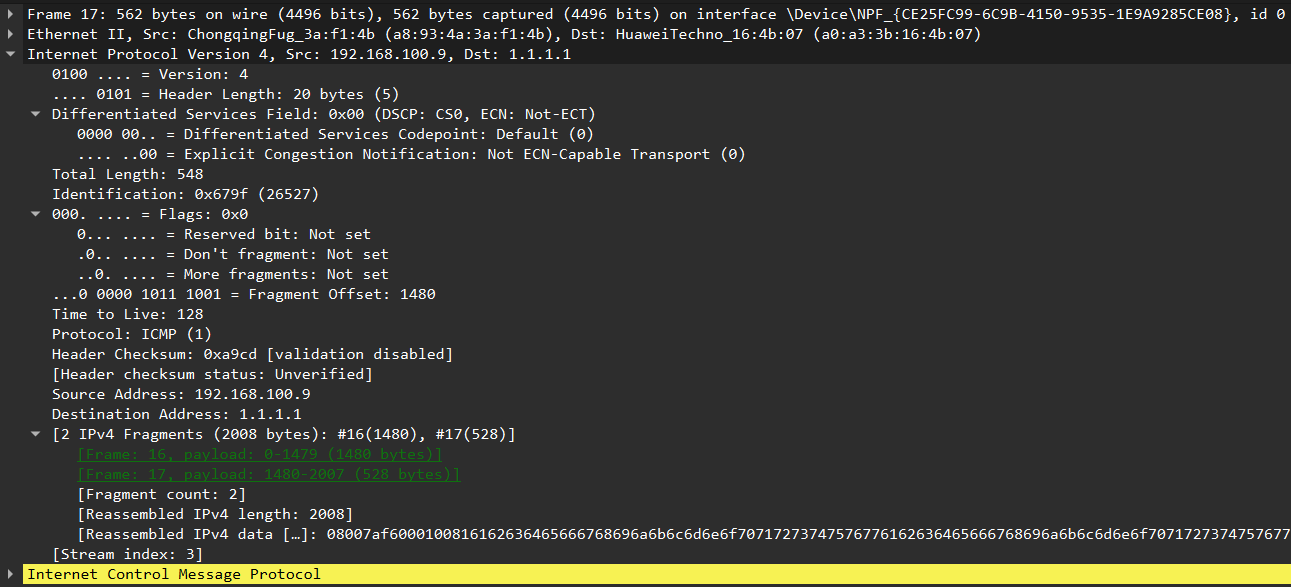
\includegraphics[width=\linewidth, height=0.45\linewidth]{screenshot038}
			\end{minipage}\hfill
			\caption{The two fragments of the first large ping request}
			\label{11}
		\end{figure}
		
		As we can see the packets in this scenario are also fragmented into two fragments. All of the requests for both DNS servers ended up in a time out.
		
		
		\section{Ad-hoc On-Demand Distance Vector Routing}
		
		\subsection{Simulation Setup}
		
		\begin{itemize}
			\item \textbf{Application Parameters:}
			
			\begin{itemize}
				\item[-] Run a \textit{PingApp} on each source node to send packets to the destination.
				
				\item[-] Configure the packet interval to \textbf{1 second}.
				
				\item[-] Log ping replies and packet loss for analysis.
				
			\end{itemize}
			
			In the following figures the codes used in \textit{.ini} and \textit{.ned} files are provided.
			
			\begin{figure}[!h]
				\centering
				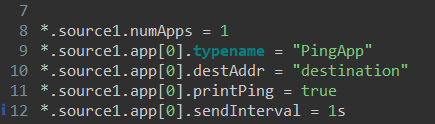
\includegraphics[width=0.7\linewidth]{screenshot039}
				\caption{The code used in the \textit{.ini} file}
				\label{fig:screenshot039}
			\end{figure}
			
			\pagebreak
			
			This code runs a \textbf{PingApp} on the source and configures the packet interval to 1s.
			
			\begin{figure}[!h]
				\centering
				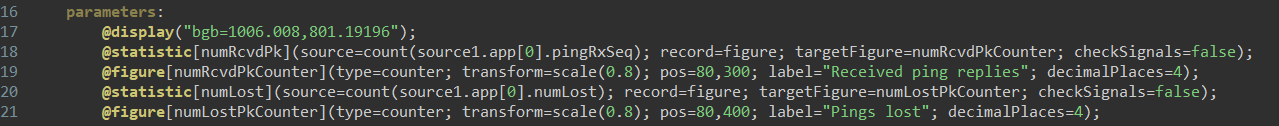
\includegraphics[width=0.7\linewidth]{screenshot040}
				\caption{The code used in the \textit{.ned} file}
				\label{fig:screenshot040}
			\end{figure}
			
			This part of the code is responsible for logging ping replies and packet loss.
			
			
			\item \textbf{Mobility Configuration:}
			
			\begin{itemize}
				\item[-] Use \textit{LinearMobility} for \textit{Router1} and \textit{Router2}.
					
				\item[-] Configure the mobility constraint area to limit node movement vertically with a constant speed (\textbf{10 m/s}).
				
				\item[-] Use the following constraints:
				
				\begin{itemize}
					\item[*] *.aodvRouter1.mobility.constraintAreaMinY = 50m
					
					\item[*] *.aodvRouter1.mobility.constraintAreaMaxY = 350m
					
					\item[*] *.aodvRouter2.mobility.constraintAreaMinY = 50m
					
					\item[*] *.aodvRouter2.mobility.constraintAreaMaxY = 350m
					
				\end{itemize}
				
			\end{itemize}
			
			\begin{figure}[!h]
				\centering
				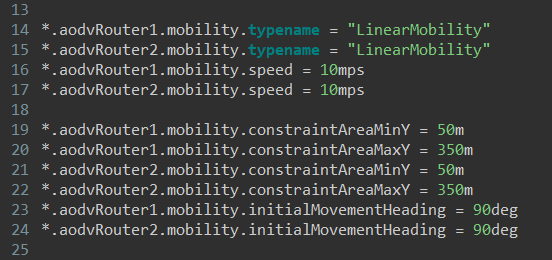
\includegraphics[width=0.7\linewidth]{screenshot041}
				\caption{The code used in the \textit{.ini} file}
				\label{fig:screenshot041}
			\end{figure}
			
			The code in the preceding figure is used to set \textit{LinearMobility} to the needed routers and also configure the mobility in a way that makes sure the routers move vertically with a constant speed of 10 m/s.
			
			We can also wee that the proper constraints are set for the mobility of routers 1 and 2.
			
			\item \textbf{Communication Range:}
			
			\begin{itemize}
				\item[-] Set the transmitter power of all nodes to \textbf{1 mW}.
				
				\item[-] Display communication ranges for all nodes to visualize network connectivity.
				
			\end{itemize}
			
			\begin{figure}[!h]
				\centering
				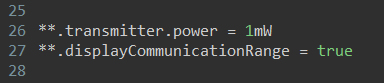
\includegraphics[width=0.7\linewidth]{screenshot042}
				\caption{The code used in the \textit{.ini} file}
				\label{fig:screenshot042}
			\end{figure}
			
			\pagebreak
			
			This part of the code sets the transmitter power of all the nodes to 1 mW and makes sure the communication range of each node is visible in the simulation.
			
			\item \textbf{Visualizer Configuration:}
			
			\begin{itemize}
				\item[-] Enable visualization of routing tables, network paths, and data links to better understand protocol dynamics.
				
				\item[-] Include counters to record the number of ping replies received and packets lost for each source.
				
				\item[-] Visualize these metrics during the simulation for real-time monitoring.
				
			\end{itemize}
			
			\begin{figure}[!h]
				\centering
				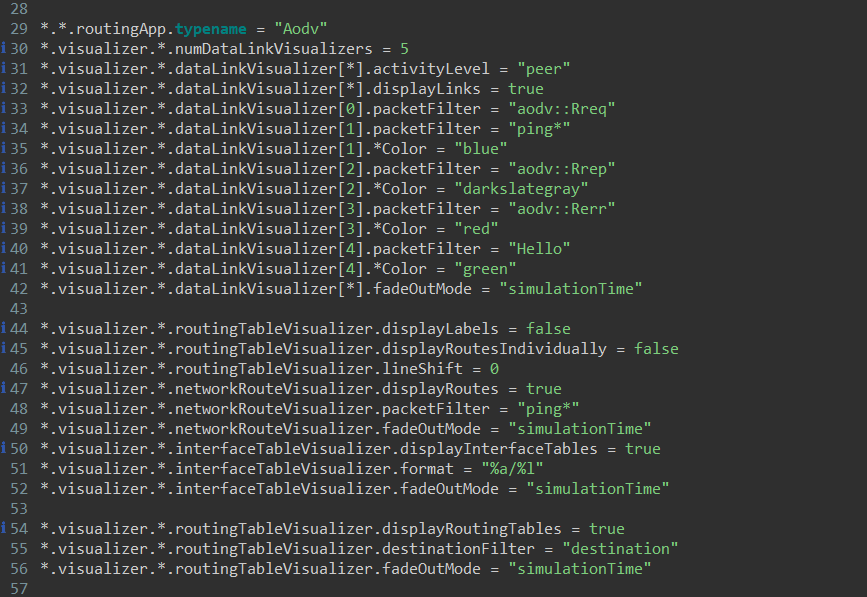
\includegraphics[width=0.68\linewidth]{screenshot043}
				\caption{The code used in the \textit{.ini} file}
				\label{fig:screenshot043}
			\end{figure}
			
			The code in the figure presented in the next page enables the visualization of the data link activity, routing tables and network routing. It is also used to set the routing protocol to AODV.
			
		\end{itemize}
		
		\begin{figure}[!h]
			\centering
			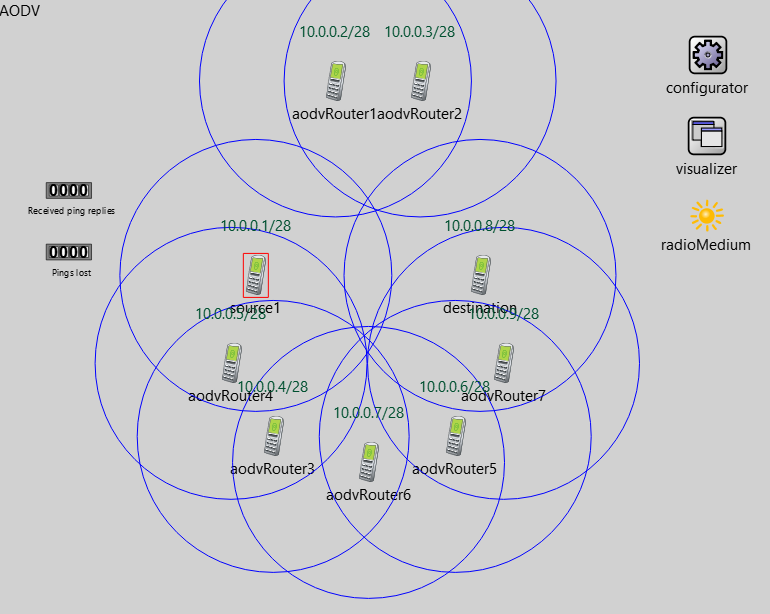
\includegraphics[width=0.68\linewidth]{screenshot044}
			\caption{The description of the Network in the simulation}
			\label{fig:screenshot044}
		\end{figure}
		
		\pagebreak
		
		\subsection{Questions}
		
		\begin{enumerate}
			\item Explain, with a screenshot, how the path is created and how the first ping packet is sent.
			
			The screenshots provided in this page and the following page demonstrate the creation of path and also shows how the first ping packet is sent.
			
			\begin{figure}[!htb]
				\begin{minipage}{0.49\textwidth}
					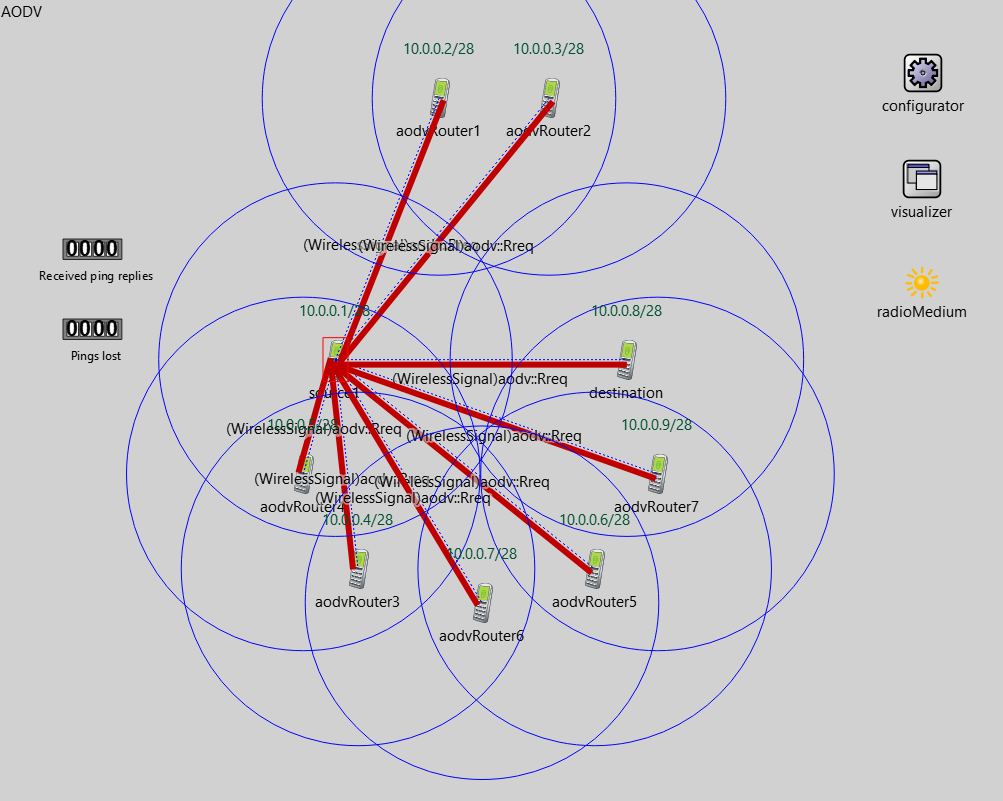
\includegraphics[width=\linewidth]{screenshot049}
				\end{minipage}\hfill
				\begin{minipage}{0.49\textwidth}
					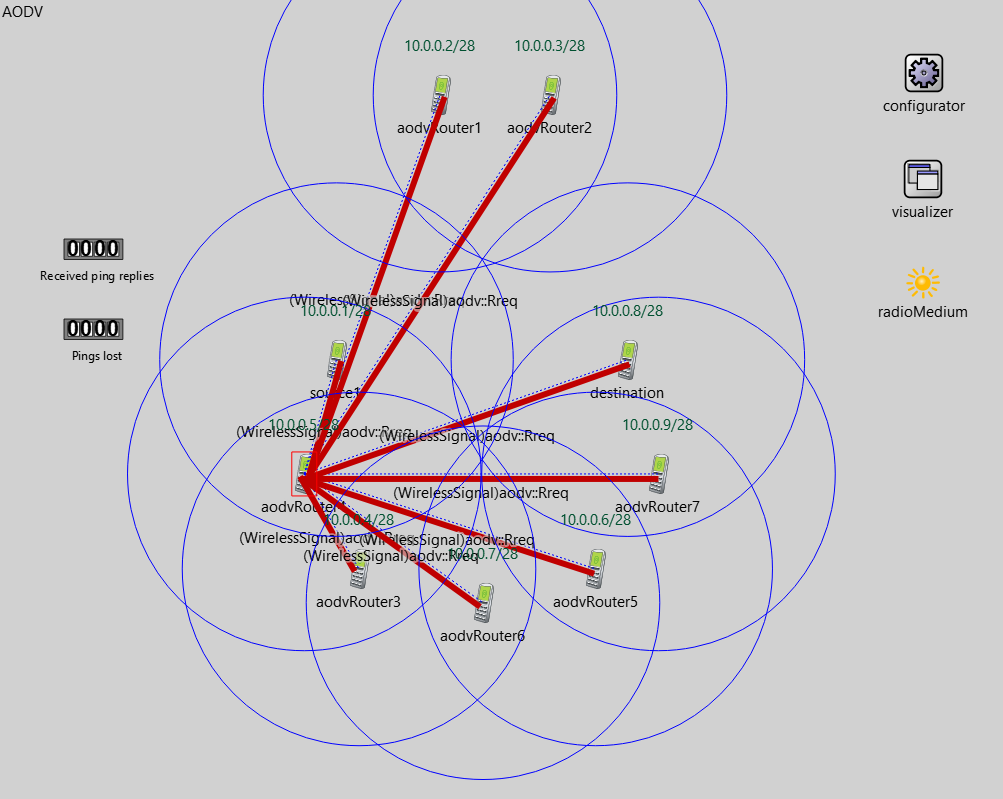
\includegraphics[width=\linewidth]{screenshot050}
				\end{minipage}\hfill
				\\\\
				
				\begin{minipage}{0.49\textwidth}
					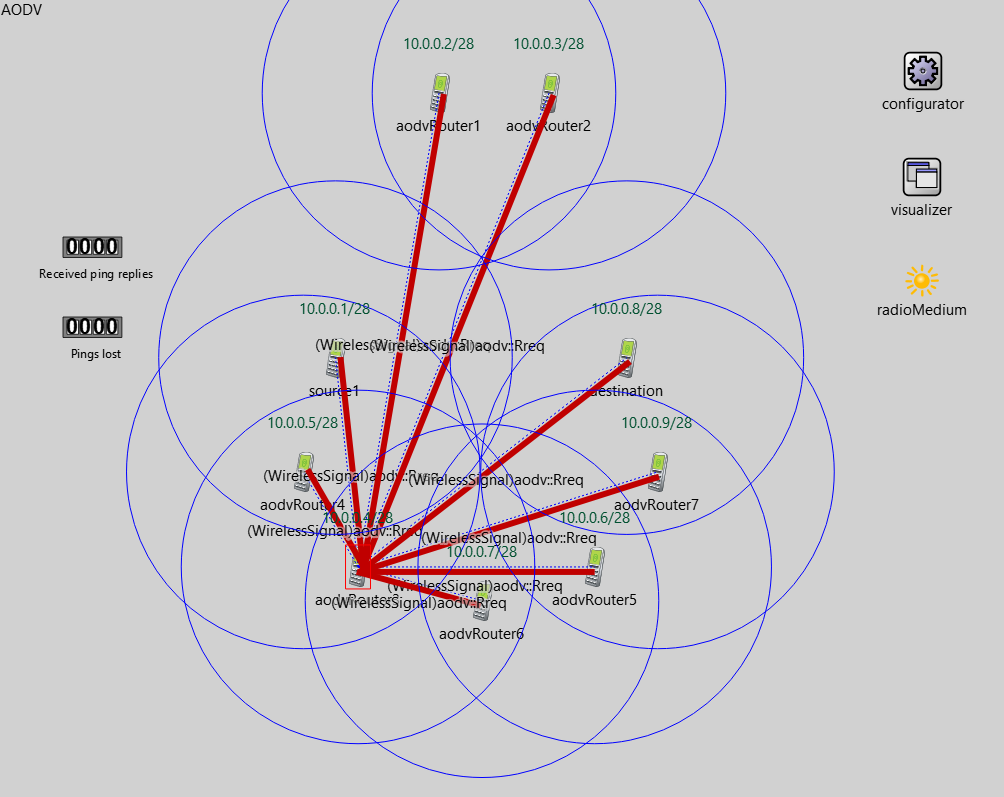
\includegraphics[width=\linewidth]{screenshot051}
				\end{minipage}\hfill
				\begin{minipage}{0.49\textwidth}
					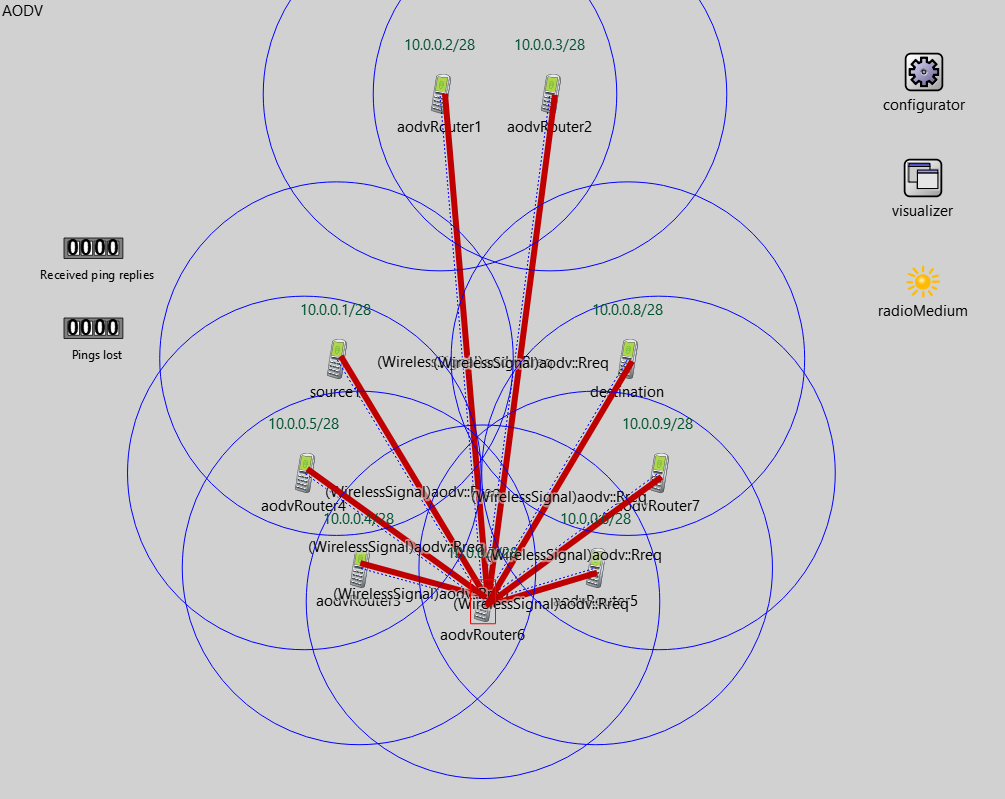
\includegraphics[width=\linewidth]{screenshot052}
				\end{minipage}\hfill
				\\\\
				
				\begin{minipage}{0.49\textwidth}
					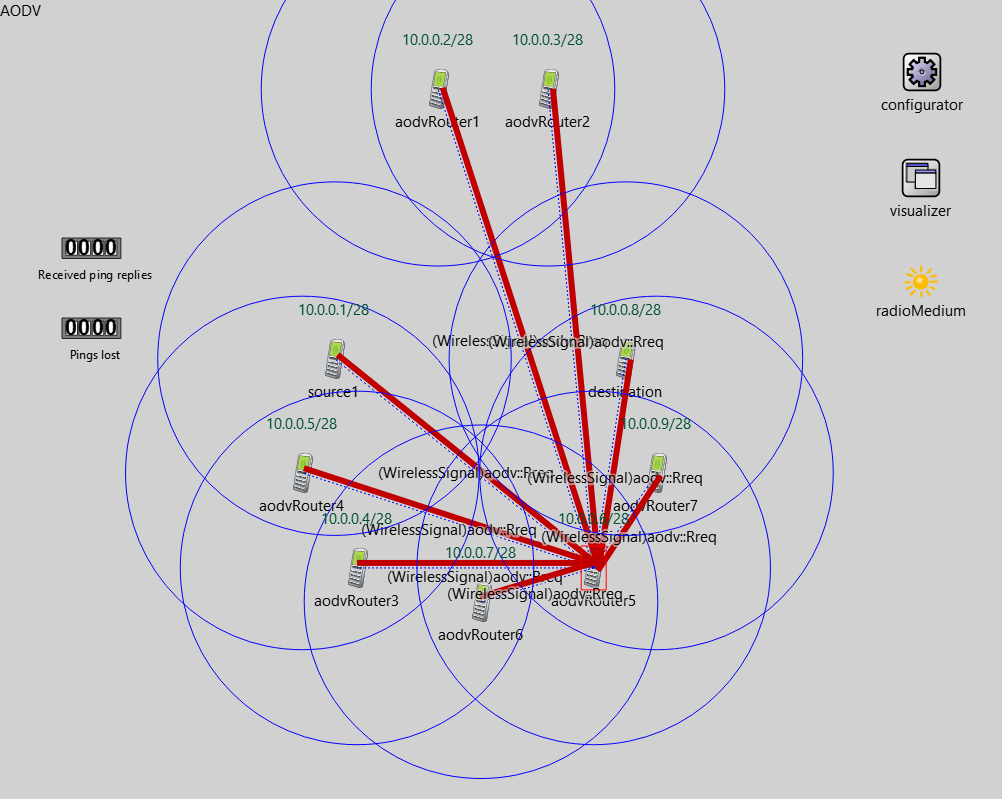
\includegraphics[width=\linewidth]{screenshot053}
				\end{minipage}\hfill
				\begin{minipage}{0.49\textwidth}
					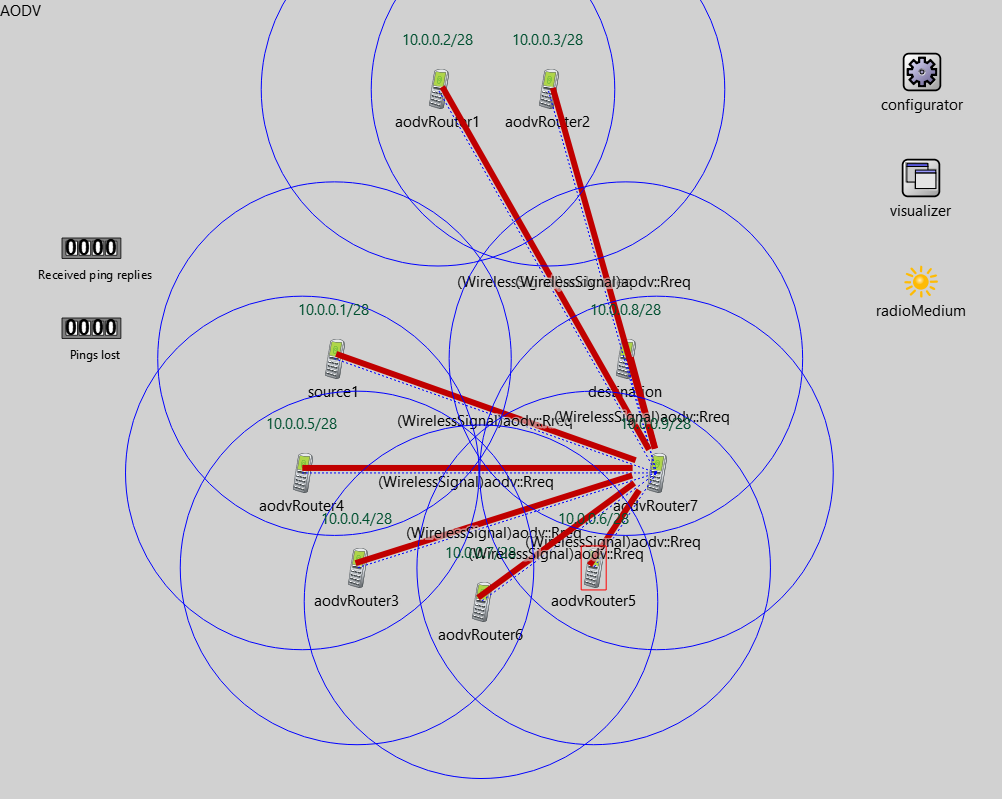
\includegraphics[width=\linewidth]{screenshot054}
				\end{minipage}\hfill
			\end{figure}
			
			\pagebreak
			
			When a node wants to send a packet, and it doesn’t know the route to the destination, it initiates route discovery, by sending an RREQ multicast message. The neighboring nodes record where the message came from and forward it to their neighbors until the message gets to the destination node. The destination node replies with an RREP, which gets back to the source on the reverse path along which the RREQ came. Forward routes are set up in the intermediate nodes as the RREP travels back to the source. An intermediate node can also send an RREP in reply to a received RREQ if it knows the route to the destination, thus nodes can join an existing route. When the RREP arrives at the source, and the route is created, communication can begin between the source and the destination.
			
			\begin{figure}[!htb]
				\begin{minipage}{0.48\textwidth}
					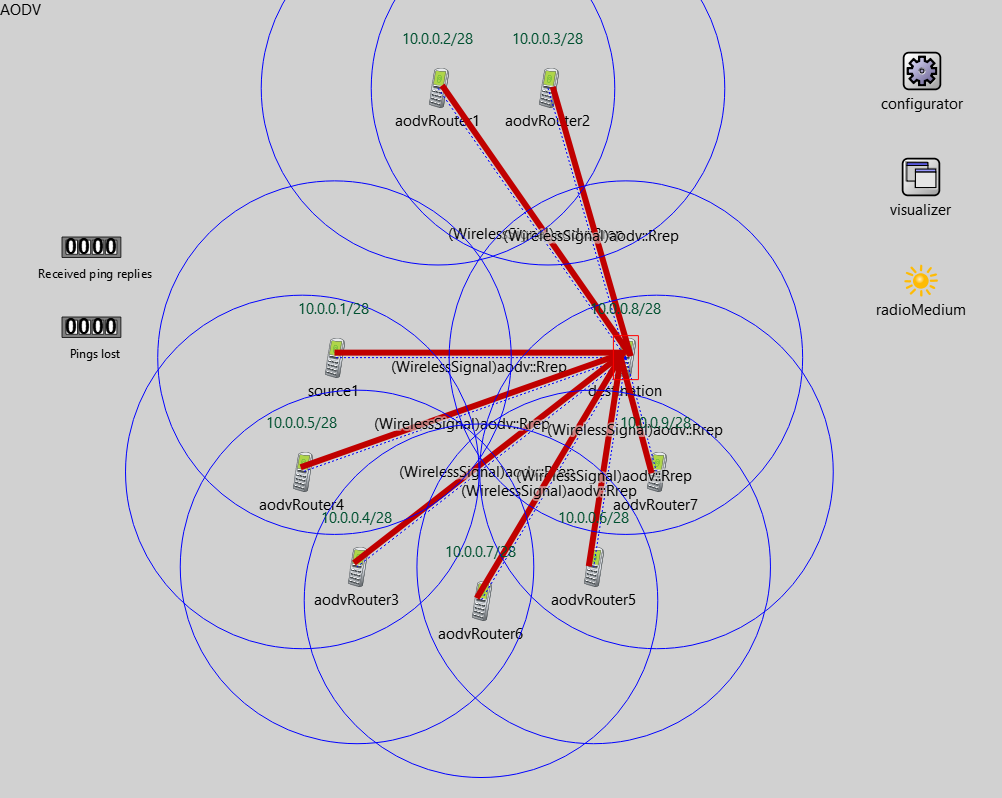
\includegraphics[width=\linewidth]{screenshot055}
				\end{minipage}\hfill
				\begin{minipage}{0.48\textwidth}
					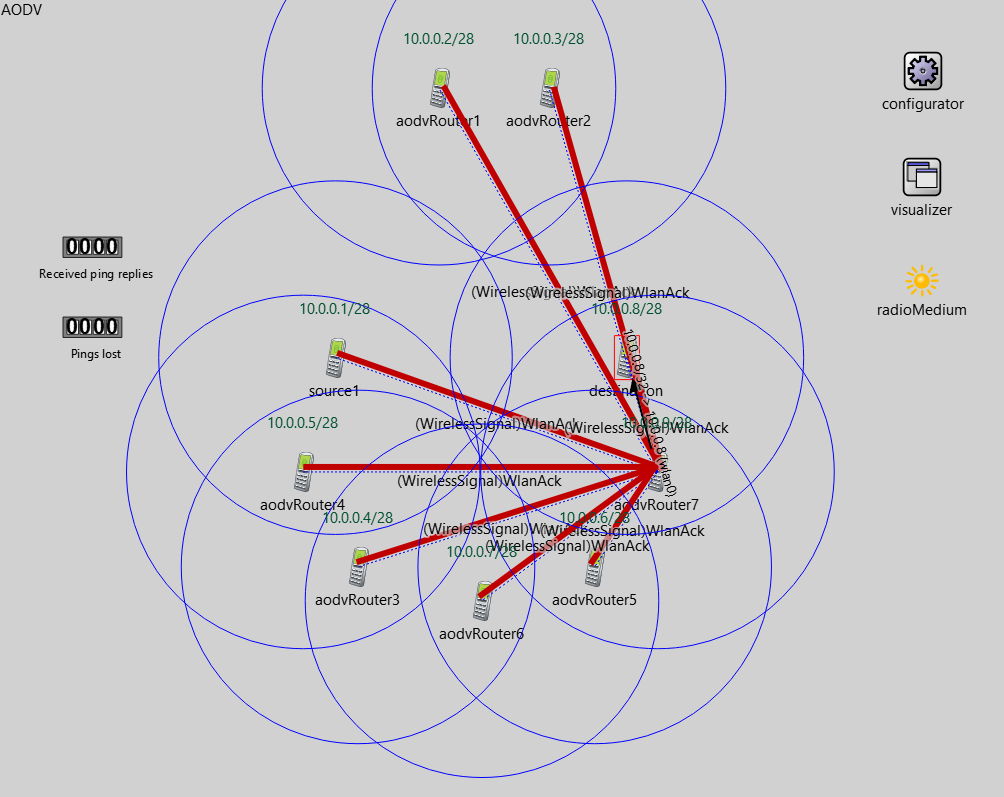
\includegraphics[width=\linewidth]{screenshot056}
				\end{minipage}\hfill
				\\\\
				\begin{minipage}{0.48\textwidth}
					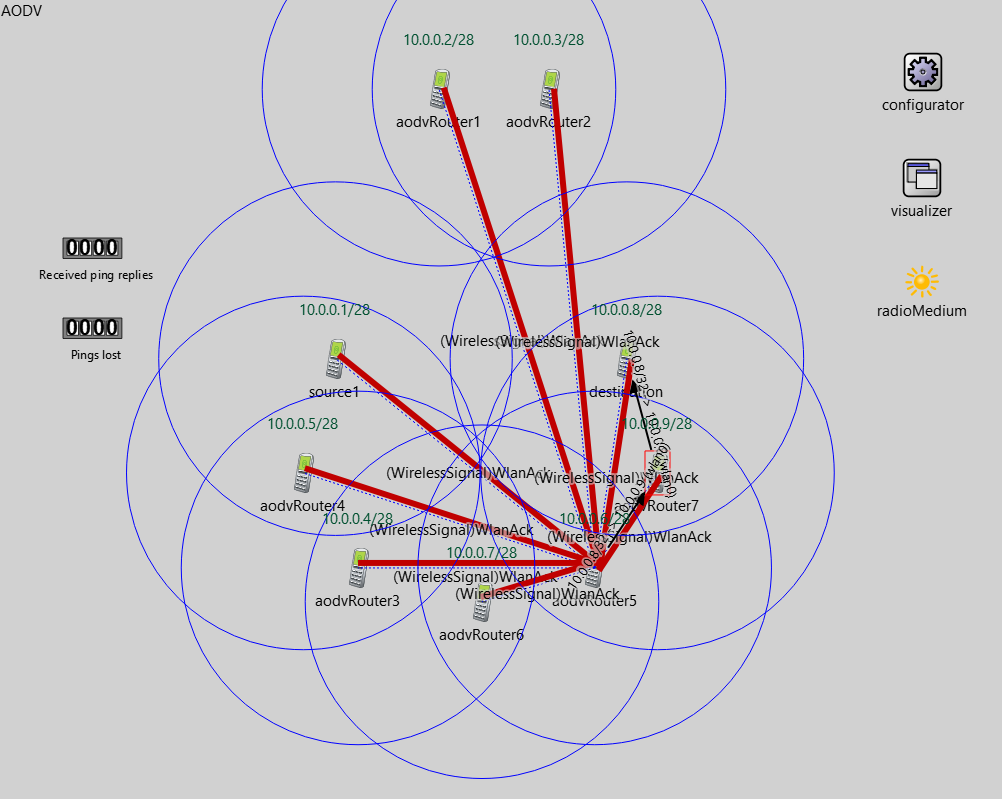
\includegraphics[width=\linewidth]{screenshot057}
				\end{minipage}\hfill
				\begin{minipage}{0.48\textwidth}
					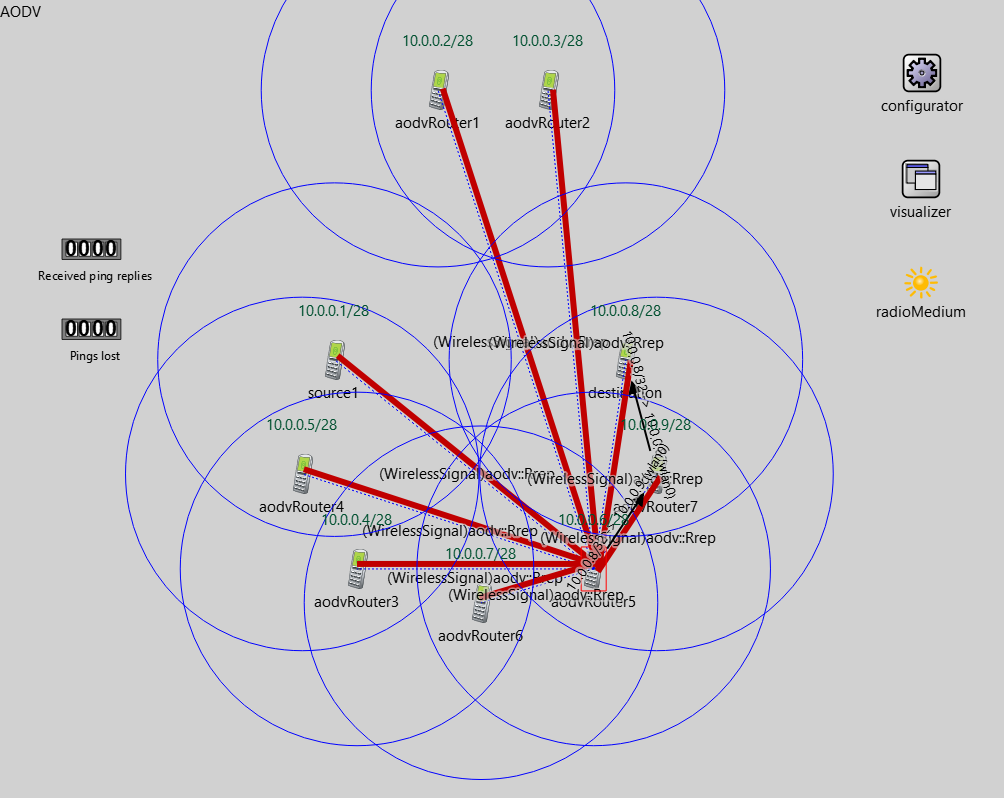
\includegraphics[width=\linewidth]{screenshot058}
				\end{minipage}\hfill
				\\\\
				\begin{center}
				\begin{minipage}{0.48\textwidth}
					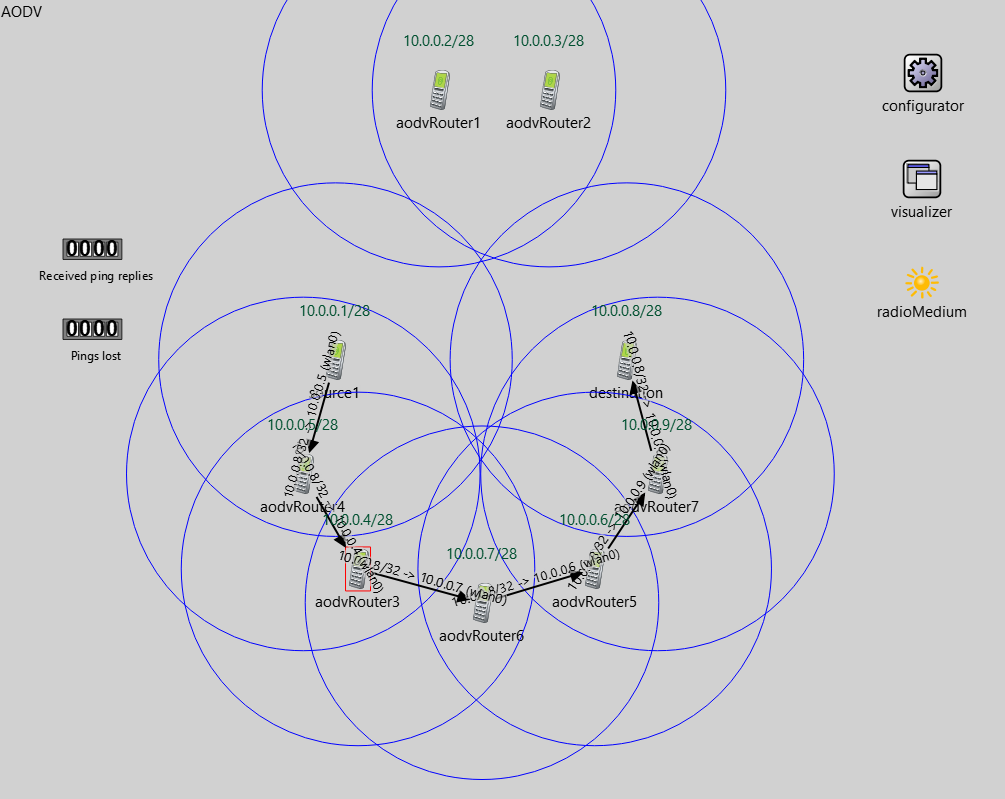
\includegraphics[width=\linewidth]{screenshot045}
				\end{minipage}\hfill
				\end{center}
				\caption{The process of path determination}
				\label{11}
			\end{figure}
			
			\pagebreak
			
			\begin{figure}[!h]
				\centering
				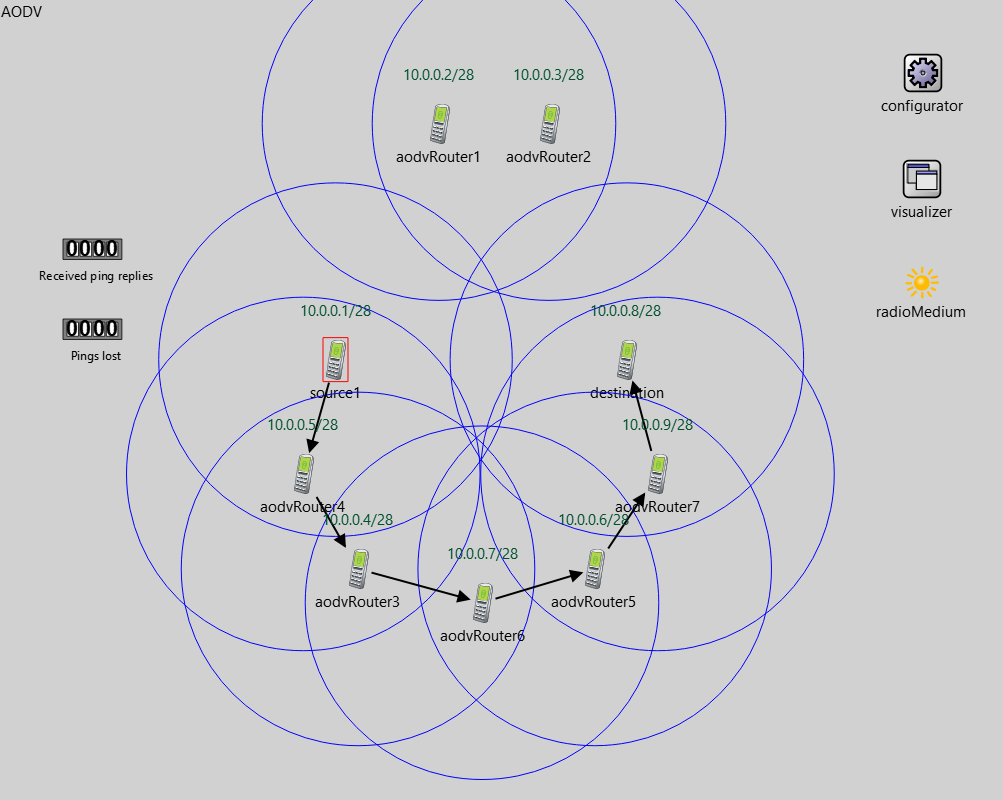
\includegraphics[width=0.7\linewidth]{screenshot048}
				\caption{The structure of the path}
				\label{fig:screenshot044}
			\end{figure}
			
			\item explore the AODV router parameters in INET by answering the following \footnote{answers to this question were obtained from \href{https://doc.omnetpp.org/inet/api-4.4.0/neddoc/inet.routing.aodv.Aodv.html}{INET documentation} and \href{https://datatracker.ietf.org/doc/rfc3561/}{RFC 3561}}:
			
			\begin{itemize}
				\item[(a)] Why do we need jitter for broadcasts, and how does it help prevent collisions?
				
				In AODV, broadcasts are critical for operations like route discovery, where Route Request (RREQ) messages are sent to all nodes within range. However, in wireless ad-hoc networks, simultaneous transmissions from multiple nodes can lead to collisions, where signals interfere and messages are lost. To mitigate this, AODV incorporates a jitter mechanism, which introduces a small random delay before transmitting broadcast messages.
				
				The INET documentation for the AODV router specifies the following parameters related to jitter:
				
				\textit{maxJitter}: Set to 5 milliseconds by default.
				
				\textit{jitter}: Defined as uniform(0ms, maxJitter).
				
				\item[(b)] Why is the initial Time-To-Live (TTL) value set low, and why is it gradually incremented?
				
				The INET implementation provides specific parameters for TTL management:
				
				\textbf{ttlStart}: Set to 2, indicating the initial TTL value for a route request.
				
				\textbf{ttlIncrement}: Set to 2, the value by which TTL is increased for each retransmission.
				
				\textbf{ttlThreshold}: Set to 7, the maximum TTL before the network diameter is used for broadcasting.
				
				\textbf{localAddTTL}: Set to 2, used for calculating initial TTL in local repairs.
				
				The initial TTL being set low (2 hops) suggests a strategy to limit the initial scope of route discovery to immediate neighbors or nearby nodes. This minimizes network overhead by avoiding unnecessary flooding of the entire network, which is particularly beneficial in large or dense MANETs where excessive broadcasts could lead to congestion and increased latency.
				
				\pagebreak
				
				If no route is found within this initial scope, the TTL is gradually incremented by 2 for each retransmission, expanding the search area incrementally. This process continues until the TTL reaches the threshold (7), after which the network diameter (a parameter set to 35 in INET, representing the maximum possible hops) is used. This approach ensures efficiency by first checking for routes to nearby destinations, which are more likely to be relevant in many scenarios, before expanding the search. It also aligns with AODV’s on-demand nature, where routes are discovered only when needed, reducing unnecessary traffic.
				
				\item[(c)] Under what conditions is a route deleted from the routing table, and what parameters influence this process?
				
				The conditions for route deletion include:
				
				\textbf{Route Expiration}: Each route has a lifetime, and if it is not refreshed or used within this period, it is considered expired and deleted. This prevents stale routes from being used, which is crucial in dynamic MANETs where topology changes frequently.
				
				\textbf{Link Break Detection}: If a node detects a link break along an active route (e.g., due to node movement or failure), it generates a Route Error (RERR) message. This message is sent to the source node and any other nodes using the route, prompting them to invalidate and eventually delete the route from their tables.
				
				\textbf{Route Not Needed}: While less explicitly stated, routes may also be deleted if they are no longer needed, such as when there are no pending packets to send to that destination, to free up space in the routing table.
				
				The parameters influencing this process include:
				
				\textbf{activeRouteTimeout}: Set to 3 seconds by default, this is the time after which an active route is considered expired if not used or refreshed. It ensures routes are periodically validated, especially in the presence of Hello messages for neighbor detection.
			
				\textbf{deletePeriod}: Set to 5 * max(activeRouteTimeout, helloInterval), this determines how long an expired route is kept before being deleted. For example, if activeRouteTimeout is 3 seconds and helloInterval is 1 second, deletePeriod would be 15 seconds, allowing time for potential re-establishment.
				
				\textbf{helloInterval}: Set to 1 second by default, this parameter, along with allowedHelloLoss (set to 2), influences route maintenance. The activeRouteTimeout must be greater than allowedHelloLoss * helloInterval to prevent premature deletion.
				
			\end{itemize}
			
			\item Analyze the key packet types used in the AODV protocol during the simulation:
			
			\begin{itemize}
				\item[(a)] \textbf{Route Request (RREQ):} Examine the fields in RREQ packets, including: rreqId, hopCount, destSeqNum, ttl.
				
				\textbf{rreqId (Route Request Identifier)}:
				It is a unique identifier for the RREQ, generated by the source node and used along with the source node's IP address to uniquely identify a specific route discovery attempt.
				It prevents processing of duplicate RREQs, reducing network overhead and avoiding routing loops. When a node receives an RREQ, it checks the rreqId and source IP against its history to discard duplicates, ensuring only the first instance is processed or forwarded.
				
				\textbf{hopCount}:
				The purpose of this field is to track the number of hops the RREQ has traversed from the source to the current node.
				It helps nodes evaluate the distance to the source and build reverse routes. Each node that forwards the RREQ increments this field.It is used to select the shortest path during route discovery and to update the routing table with the freshest route (based on hop count and sequence numbers).
				
				\pagebreak
				
				\textbf{destSeqNum (Destination Sequence Number)}:
				This field represents the source node’s knowledge of the destination’s sequence number, if available, or the last known sequence number.
				It ensures route freshness and loop prevention. Nodes compare the \textit{destSeqNum} in the RREQ with their own routing table’s destination sequence number (if they have a route to the destination). A higher or equal sequence number indicates a fresher route, prompting the node to generate an RREP or forward the RREQ.
				
				\textbf{ttl (Time-To-Live)}:
				It limits the number of hops an RREQ can travel before being discarded.
				It is responsible for controlling the scope of route discovery to prevent excessive flooding. Here, the \textit{ttlStart} parameter (default 2) sets the initial TTL, which is incremented by \textit{ttlIncrement} (default 2) up to \textit{ttlThreshold} (default 7), and eventually to the network diameter (default 35). A node decrements the TTL before forwarding; if TTL reaches 0, the packet is dropped.
				
				\item[(b)] \textbf{Route Reply (RREP):} Review the fields in RREP packets.
				
				The key fields in RREP packets\footnote{obtained from INET documentaion}:
				
				\begin{table}[!h]
					\centering
					\begin{tabular}{| p{3cm} | p{10cm} |}
						\hline
						\textbf{Field} & \textbf{Description} \\\hline
						hopCount & Tracks the number of hops from the destination to the source. This helps the source choose the best (shortest) route. \\\hline
						destAddress & The IP address of the destination. \\\hline
						destSeqNum & The destination’s sequence number, indicating the freshness of the route. Helps the source determine whether to use this route. \\\hline
						lifetime & The time in milliseconds for which the route is considered valid. It’s copied into the routing table on the source side. \\\hline
					\end{tabular}
					\caption{Fields in the AODV Route Reply (RREP) Packet}
				\end{table}
				
				\item[(c)] What purpose do the Source and Destination Sequence Numbers serve in each routing packet?
				
				Key Purposes of Sequence Numbers:
				
				\textbf{Loop Prevention}: Sequence numbers make sure that newer routing information take the place of the older ones, preventing routing loops. If a node receives a packet with a lower sequence number than its current entry, it discards it.
				
				\textbf{Route Freshness}: By comparing sequence numbers, nodes select the most recent route, critical in MANETs where topology changes frequently due to mobility of the nodes.
				
				\textbf{Route Selection}: During route discovery, nodes use sequence numbers to prioritize fresher routes over older ones, even if the hop count is higher, ensuring robust routing decisions.
				
			\end{itemize}
			
			\item \textbf{activeRouteTimeout}
			
			\begin{itemize}
				\item[(a)] Does AODV always send packets through the shortest path?
				
				No.\\
				AODV prefers the shortest (least-hop) path among the available and valid routes. However when multiple RREQs reach a destination, it responds to only the first valid one, even if a later one would result in a shorter route.
				Intermediate nodes forward only the first RREQ they see, discarding duplicates (to avoid flooding loops).
				The route established is based on the first received RREQ, which is often—but not guaranteed to be the shortest.\\
				Therefore, AODV can lock into a suboptimal path if it receives an RREQ over a longer route before the optimal one arrives.
				
				\item[(b)] What is the impact of the \textit{activeRouteTimeout} parameter on the network’s ability to select a better path?
				
				The \textit{activeRouteTimeout} parameter determines how long a route remains valid. A shorter timeout (e.g., 1 second) forces more frequent route discoveries, increasing the likelihood of finding a better path but adding control overhead. A longer timeout (e.g., 10 seconds) reduces overhead by keeping routes longer, but it may delay finding better paths if the network topology changes.
				
				\item[(c)] What are the effects of using low and high values for this parameter?
				
				As explained in the previous question, a longer \textit{activeRouteTimeout} keeps routes in the routing table for a longer period, increasing the likelihood that an existing (potentially suboptimal) route is used instead of triggering a new route discovery. This can delay the discovery of a better (e.g., shorter or fresher) path, especially in dynamic networks where topology changes frequently.\\
				On the other hand, shorter \textit{activeRouteTimeout} forces routes to expire more quickly, prompting more frequent route discoveries via RREQs. This increases the chance of finding a better path (e.g., shorter or more stable) but at the cost of higher control overhead due to repeated broadcasts.
				
				\item[(d)] Simulate the network using different \textit{activeRouteTimeout} values and explain the impact.
				
				
				\textit{activeRouteTimeout} = 1 sec:
				
				The overall number of RREP and RREQ packets generated increases significantly. Also the path changes when routers 1 and 2 come closer to the source and destination and eventually the path through those routers is selected. It is observed that some ping replies come back to the source with a great delay or even do not come back and the ping packet gets lost. All in all we can say that if the \textit{activeRouteTimeout} is less than a normal value (2 or 3 seconds) instability might happen leading to packet loss or undesirable delays.
				
				\begin{figure}[!h]
					\centering
					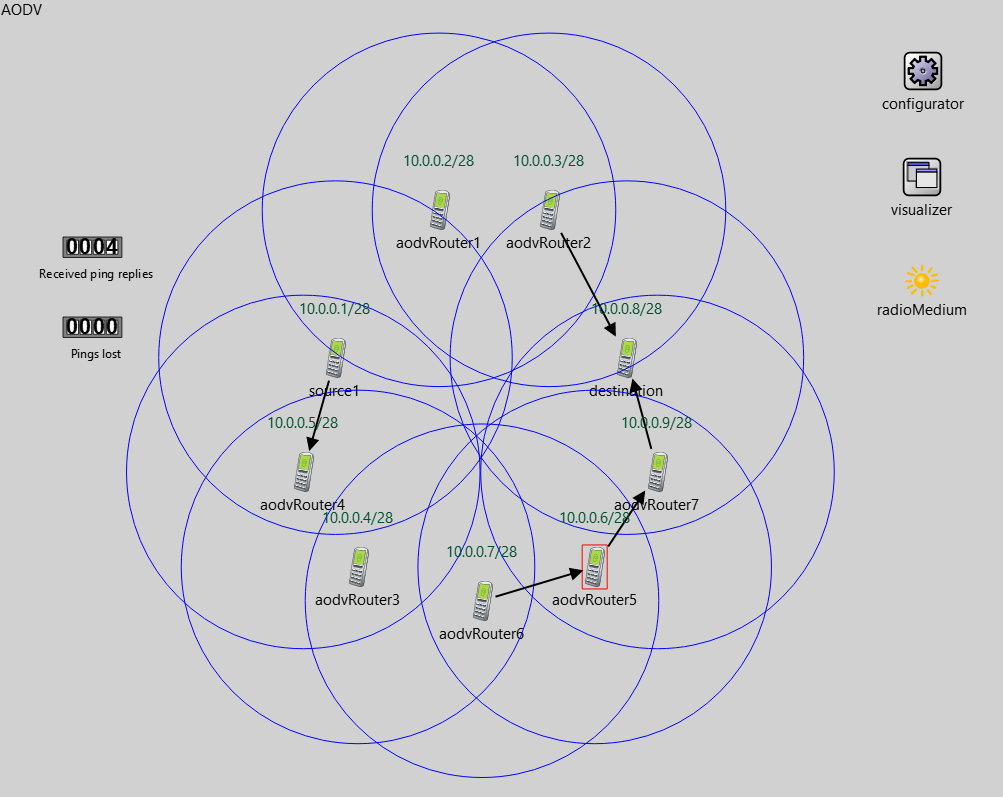
\includegraphics[width=0.5\linewidth]{screenshot061}
					\caption{The selected path changes due to the short timeout}
					\label{fig:screenshot061}
				\end{figure}
				\begin{figure}[!htb]
					\begin{minipage}{0.49\textwidth}
						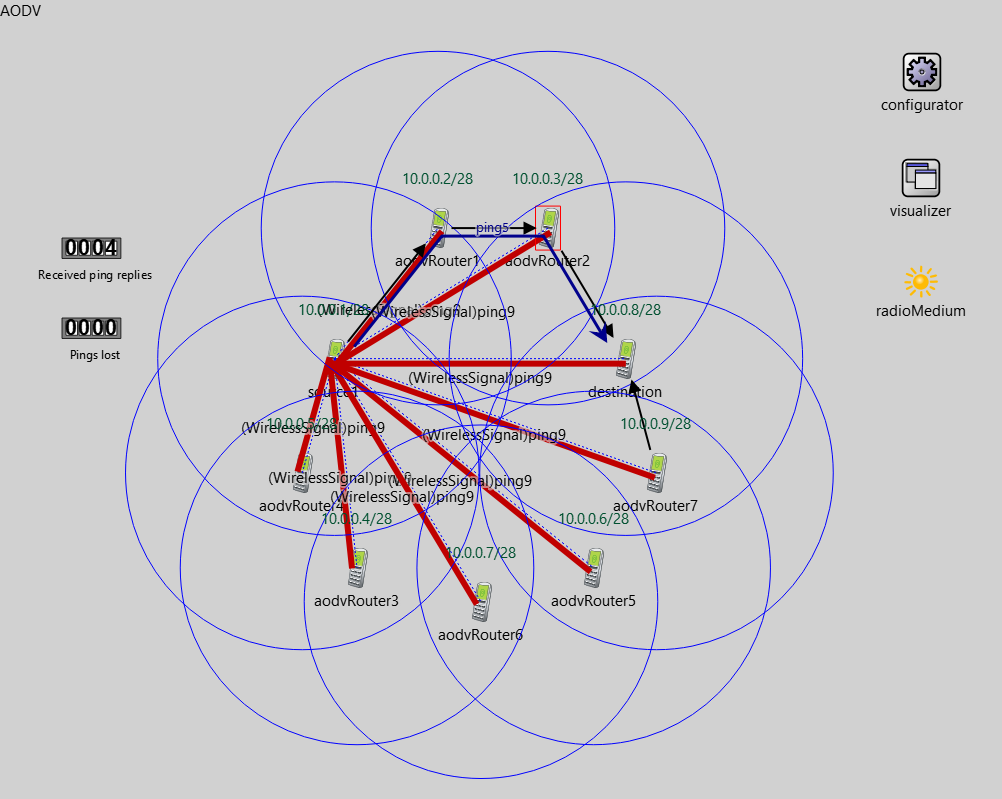
\includegraphics[width=\linewidth]{screenshot062}
						\caption{Some ping replies come back with a long delay}
					\end{minipage}\hfill
					\begin{minipage}{0.49\textwidth}
						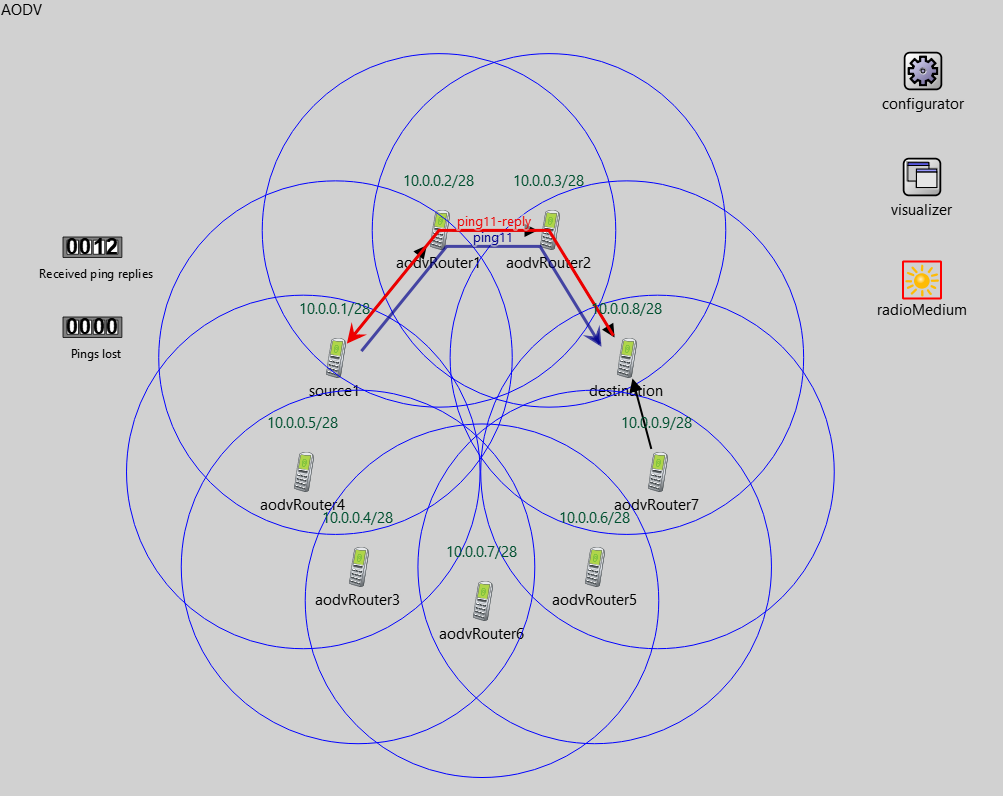
\includegraphics[width=\linewidth]{screenshot063}
						\caption{Some ping replies come back with a long delay}
					\end{minipage}\hfill
				\end{figure}
				
				\pagebreak
				
				\begin{figure}[!htb]
					\begin{minipage}{0.49\textwidth}
						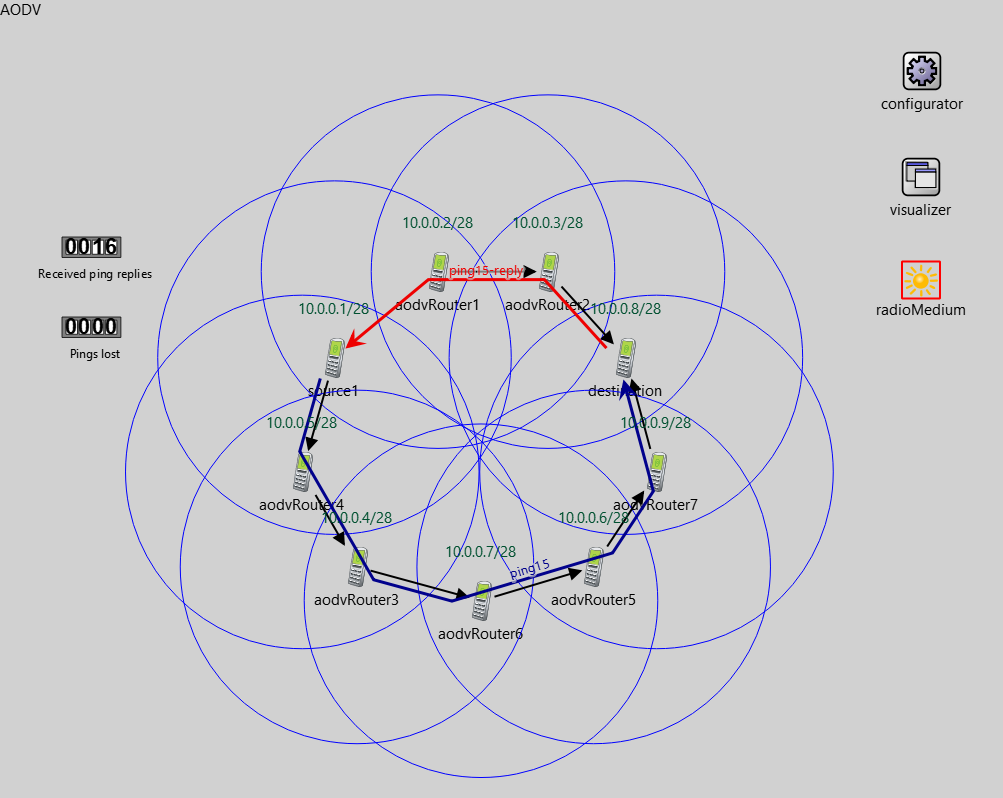
\includegraphics[width=\linewidth]{screenshot064}
						\caption{The ping and ping reply paths are not necessarily the same in this case}
					\end{minipage}\hfill
					\begin{minipage}{0.49\textwidth}
						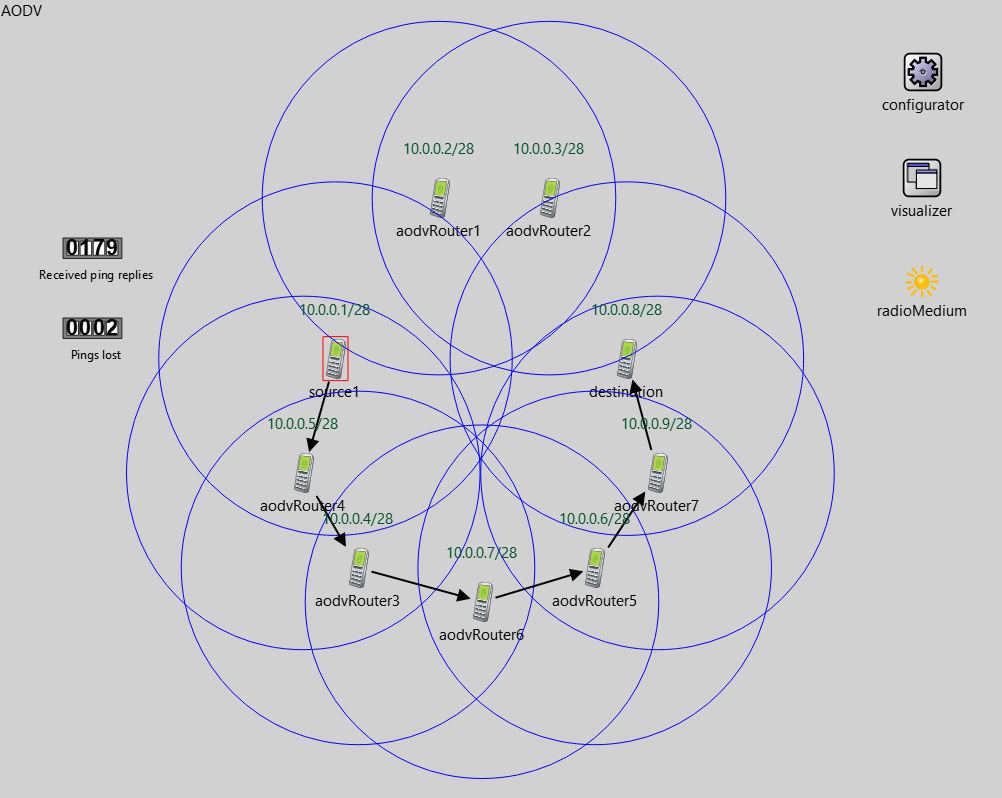
\includegraphics[width=\linewidth]{screenshot066}
						\caption{In this case we see some lost packets due to the instability}
					\end{minipage}\hfill
				\end{figure}
				
				
				\textit{activeRouteTimeout} = 10 sec:
				
				In this case, because the timeout is large the routers in the path remain valid for a much longer time and thus we see much less RREQ and RREP packets. The selected route is not always the best path and when the two upper routers come closer to the source and destination there exists a better path.
				
				\begin{figure}[!htb]
					\begin{minipage}{0.49\textwidth}
						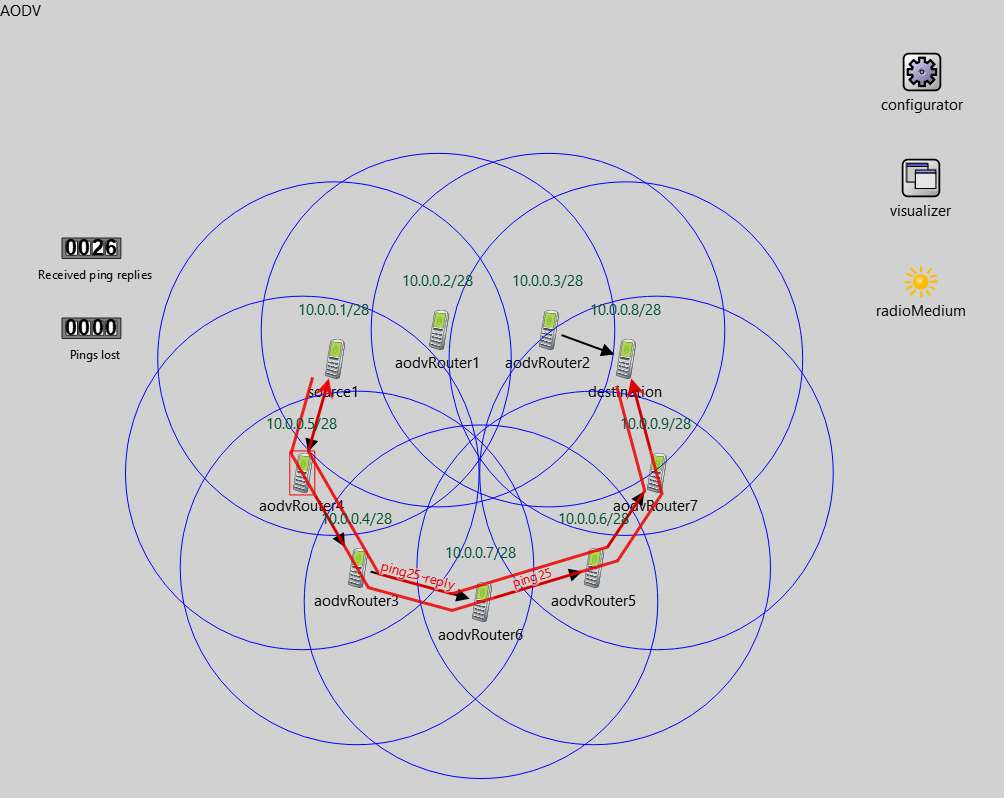
\includegraphics[width=\linewidth]{screenshot059}
						\caption{In this case the path and the router remain valid for a long time}
					\end{minipage}\hfill
					\begin{minipage}{0.49\textwidth}
						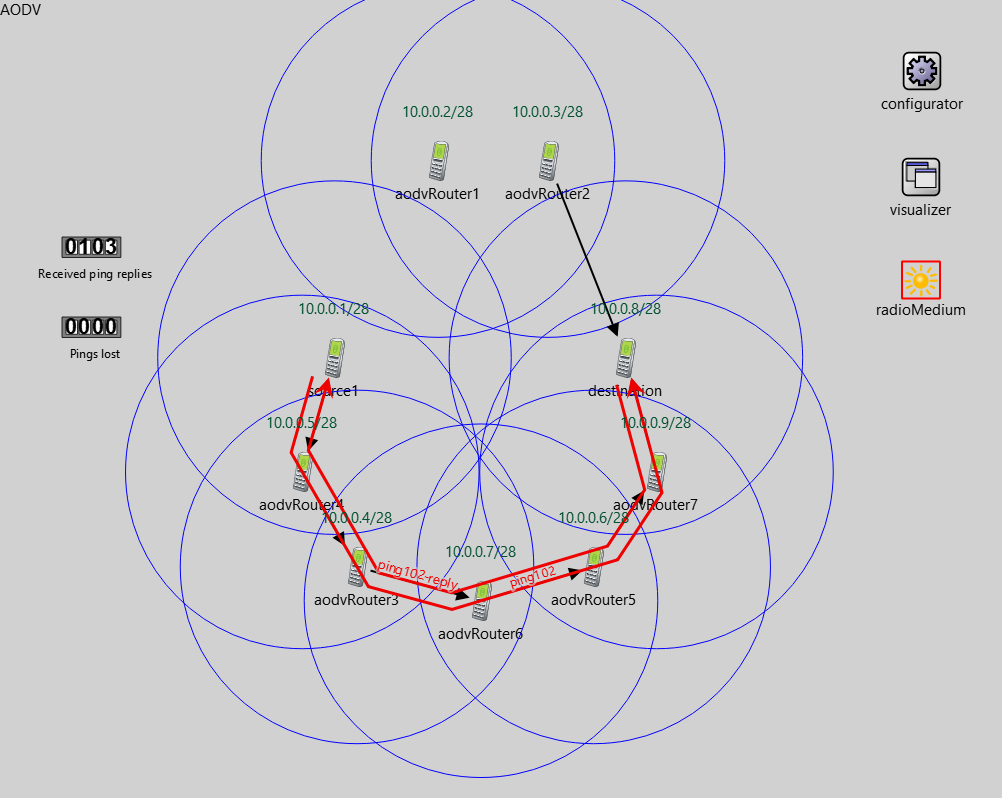
\includegraphics[width=\linewidth]{screenshot060}
						\caption{After a long time there is no lost packet and the network is stable}
					\end{minipage}\hfill
				\end{figure}
				
				
			\end{itemize}
			
			\item \textbf{Route Error (RERR)}
			
			\begin{itemize}
				\item Add mobility to \textit{Router6} in order to break the established route.
				
				\item Observe the scenarios where RERR packets are generated.
				
				As we can see in the screenshots below, after adding a 20 mps linear mobility with uniform(0$\deg$, 360$\deg$) movement heading to router6, the router starts moving until router5 stays out of its communication range. After this router6 broadcasts the ping packet several times and then eventually sends a RERR back to router3. Then the routers send the RERR packet back to the source. Following this, the routers try to find a path to send the ping packet via sending several RREQ and RREP packets until when the upper router enter the communication range of the source and destination. Afterwards the source uses the path through the upper routers and sends the ping packets.
				
				
				\pagebreak
				
				\begin{figure}[!htb]
					\begin{minipage}{0.49\textwidth}
						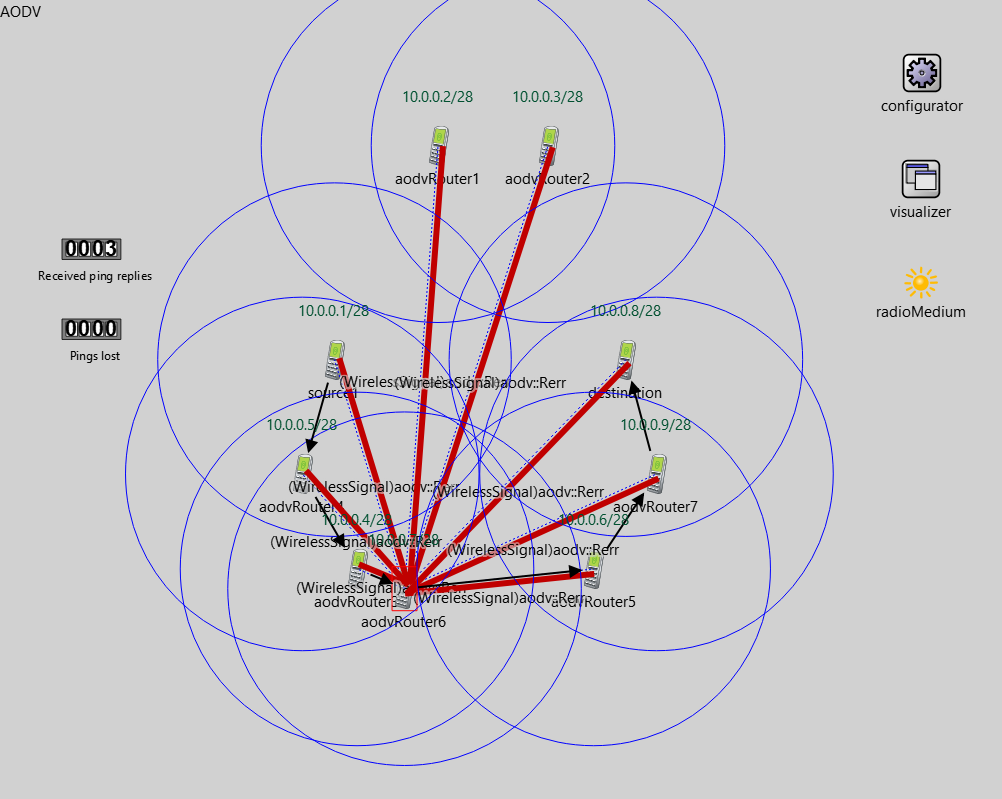
\includegraphics[width=\linewidth]{screenshot067}
						\caption{Router6 sends a RERR packet to router3 because router5 is out of its range }
					\end{minipage}\hfill
					\begin{minipage}{0.49\textwidth}
						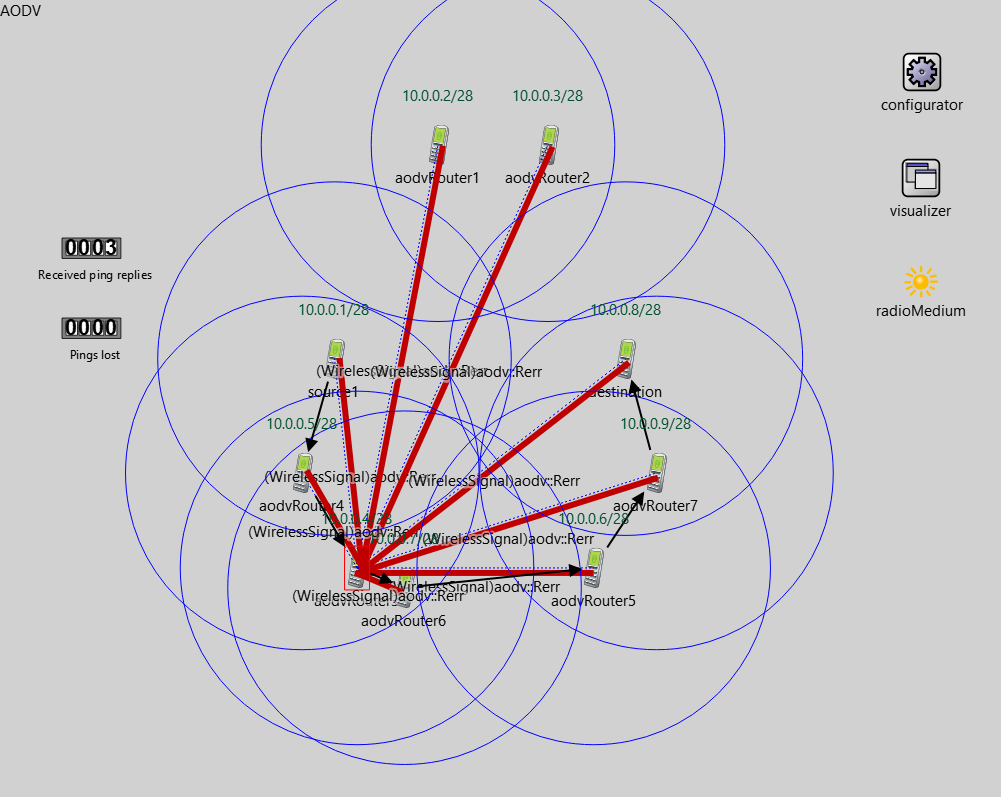
\includegraphics[width=\linewidth]{screenshot068}
						\caption{Router3 passes the RERR packet to router4 so that it would be forwarded to the source}
					\end{minipage}\hfill
				\end{figure}
				\begin{figure}[!htb]
					\begin{minipage}{0.49\textwidth}
						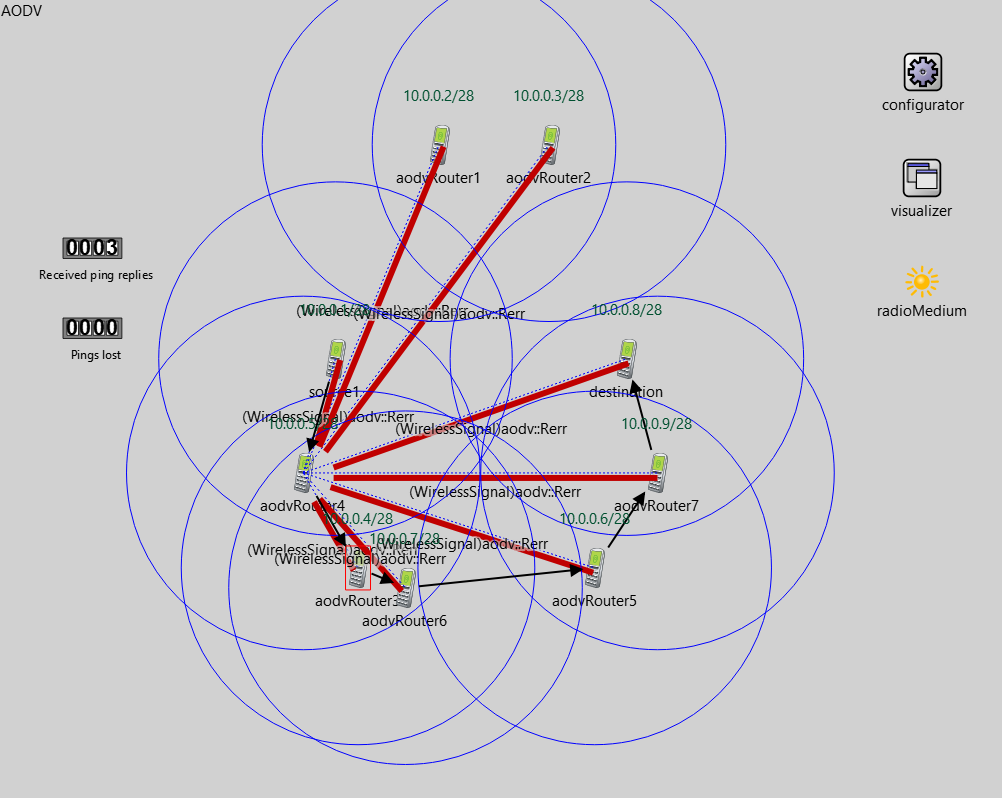
\includegraphics[width=\linewidth]{screenshot069}
						\caption{Router4 then gives the RERR packet to the source node}
					\end{minipage}\hfill
					\begin{minipage}{0.49\textwidth}
						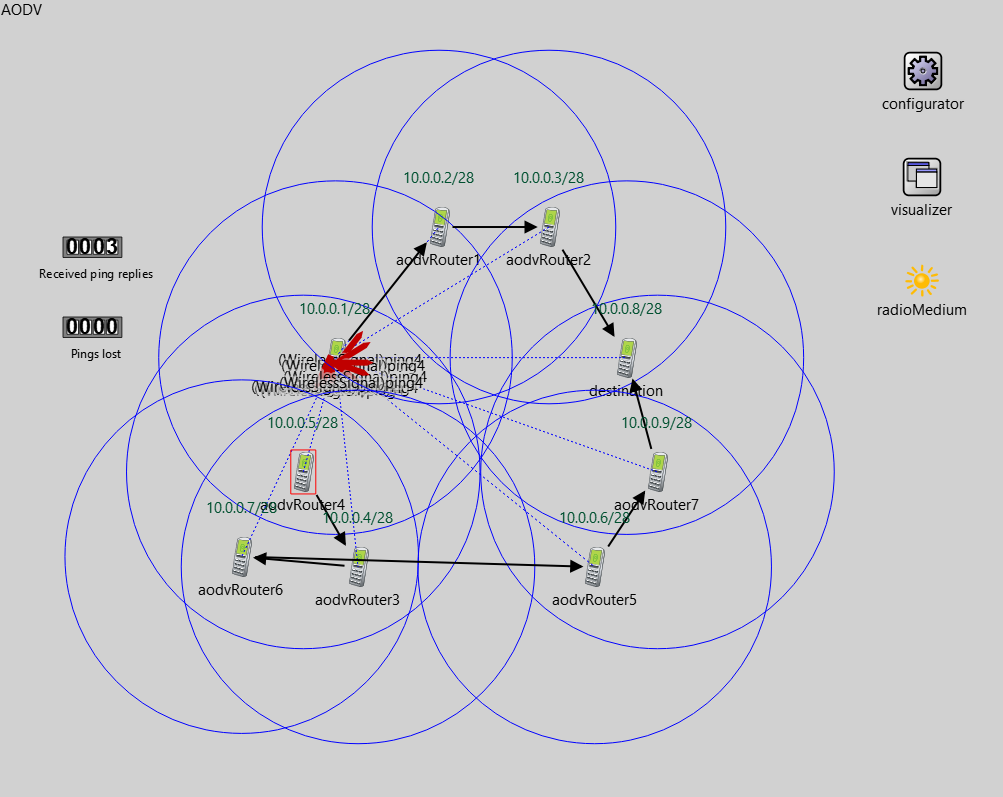
\includegraphics[width=\linewidth]{screenshot070}
						\caption{The nodes try to find a route until the upper routers get close enough}
					\end{minipage}\hfill
				\end{figure}
				
				
			\end{itemize}
			
			\item \textbf{Hello Packets}
			
			\begin{itemize}
				\item[(a)] What is the purpose of Hello packets, and why are they disabled by default in some configurations?
				
				Hello packets are small, periodic unicast or local broadcast messages that allow AODV nodes to detect the presence or absence of neighboring nodes.\\
				Hello packets let nodes confirm their 1-hop neighbors are still within range, even if no data or control traffic is being exchanged. If a node stops receiving Hello packets from a neighbor for a certain time (\textit{allowedHelloLoss} times \textit{helloInterval}), it considers the link broken and triggers RERR. Routes that rely on neighbor connectivity can be refreshed or invalidated based on Hello reception.
				
				In default AODV implementations, the protocol works with link layer detection rather than Hello packets, suggesting that alternative mechanisms can handle neighbor discovery. For instance, in networks using IEEE 802.11, link layer notifications (e.g., absence of ACKs or failure to get CTS after RTS) can detect link breakages, reducing the need for Hello packets. Besides that, disabling Hello packets can reduce network overhead, saving bandwidth and processing power, which is particularly beneficial in resource-constrained environments like MANETs.
				
				\pagebreak
				
				\item[(b)] Modify the ping app to observe the effect of hello packets. Configure the ping app to ping 3 times initially.
				After 3 pings, do not ping again until the destination moves back. Once the destination has moved back, ping
				again.
				
				
				
				\item[(c)] Are Hello packets forwarded like RREQ messages?
				
				No.
				Hello packets are not forwarded like RREQ messages.
				Hello messages are broadcast with TTL=1 which means they are only received by immediate neighbors and are not propagated further through the network.
				
			\end{itemize}
			
		\end{enumerate}
		
		
		
\end{document}